\documentclass[preprint,12pt,authoryear]{elsarticle}

\usepackage{amsmath}
\usepackage{booktabs}
\usepackage{array}
\newcolumntype{L}[1]{>{\raggedright\arraybackslash}p{#1}}
\usepackage{graphicx}
\usepackage[hidelinks]{hyperref}
\usepackage{lineno}
\linenumbers

% written by build_values_figures.py, do not edit
\newcommand{\vCalBalAuc}{0.50}
\newcommand{\vCalBalCauc}{0.50}
\newcommand{\vCalBalSauc}{0.49}
\newcommand{\vCalDCA}{-0.004}
\newcommand{\vCalDCAHi}{0.000}
\newcommand{\vCalDCALo}{-0.011}
\newcommand{\vCalDSA}{-0.007}
\newcommand{\vCalDSAHi}{0.000}
\newcommand{\vCalDSALo}{-0.018}
\newcommand{\vCalDSC}{-0.004}
\newcommand{\vCalDSCHi}{0.000}
\newcommand{\vCalDSCLo}{-0.011}
\newcommand{\vCalLossAuc}{0.050}
\newcommand{\vCalLossCauc}{0.050}
\newcommand{\vCalLossSauc}{0.051}
\newcommand{\vCalPrefAuc}{0.00}
\newcommand{\vCalPrefCauc}{0.00}
\newcommand{\vCalPrefSauc}{0.00}
\newcommand{\vCalRelAuc}{0.56}
\newcommand{\vCalRelCauc}{0.56}
\newcommand{\vCalRelSauc}{0.57}
\newcommand{\vCalTruthEnv}{0.53}
\newcommand{\vMcBalAuc}{0.61}
\newcommand{\vMcBalCauc}{0.73}
\newcommand{\vMcBalSauc}{0.67}
\newcommand{\vMcDCA}{0.223}
\newcommand{\vMcDCAHi}{0.242}
\newcommand{\vMcDCALo}{0.204}
\newcommand{\vMcDSA}{0.099}
\newcommand{\vMcDSAHi}{0.112}
\newcommand{\vMcDSALo}{0.087}
\newcommand{\vMcDSC}{-0.124}
\newcommand{\vMcDSCHi}{-0.106}
\newcommand{\vMcDSCLo}{-0.143}
\newcommand{\vMcDraws}{5}
\newcommand{\vMcLossAuc}{0.047}
\newcommand{\vMcLossCauc}{0.023}
\newcommand{\vMcLossSauc}{0.035}
\newcommand{\vMcPrefAuc}{0.17}
\newcommand{\vMcPrefCauc}{0.42}
\newcommand{\vMcPrefSauc}{0.27}
\newcommand{\vMcRelAuc}{0.58}
\newcommand{\vMcRelCauc}{0.29}
\newcommand{\vMcRelSauc}{0.43}
\newcommand{\vMcTruthEnv}{0.78}
\newcommand{\vTwBalAuc}{0.72}
\newcommand{\vTwBalCauc}{0.76}
\newcommand{\vTwBalSauc}{0.73}
\newcommand{\vTwDCA}{0.135}
\newcommand{\vTwDCAHi}{0.171}
\newcommand{\vTwDCALo}{0.100}
\newcommand{\vTwDSA}{0.031}
\newcommand{\vTwDSAHi}{0.044}
\newcommand{\vTwDSALo}{0.018}
\newcommand{\vTwDSC}{-0.104}
\newcommand{\vTwDSCHi}{-0.076}
\newcommand{\vTwDSCLo}{-0.135}
\newcommand{\vTwLossAuc}{0.035}
\newcommand{\vTwLossCauc}{0.021}
\newcommand{\vTwLossSauc}{0.033}
\newcommand{\vTwPrefAuc}{0.37}
\newcommand{\vTwPrefCauc}{0.55}
\newcommand{\vTwPrefSauc}{0.41}
\newcommand{\vTwRelAuc}{0.33}
\newcommand{\vTwRelCauc}{0.19}
\newcommand{\vTwRelSauc}{0.31}
\newcommand{\vTwTruthEnv}{0.79}
\newcommand{\vaggAgree}{98.6}
\newcommand{\vaggKappa}{0.91}
\newcommand{\valBestCi}{0.864}
\newcommand{\valBestCiHi}{0.873}
\newcommand{\valBestCiLo}{0.854}
\newcommand{\valBestName}{RF}
\newcommand{\valBlockNull}{0.757}
\newcommand{\valBlockRep}{0.850}
\newcommand{\valDiff}{0.010}
\newcommand{\valNullCi}{0.874}
\newcommand{\valNullCiHi}{0.883}
\newcommand{\valNullCiLo}{0.865}
\newcommand{\valTempNull}{0.874}
\newcommand{\valTempNullSeventeen}{0.877}
\newcommand{\valTempRep}{0.864}
\newcommand{\vapBaseFive}{0.302}
\newcommand{\vapBaseFiveHi}{0.355}
\newcommand{\vapBaseFiveLo}{0.248}
\newcommand{\vapBaseTen}{0.255}
\newcommand{\vapBaseTenHi}{0.301}
\newcommand{\vapBaseTenLo}{0.209}
\newcommand{\vapBaseTwenty}{0.192}
\newcommand{\vapBaseTwentyHi}{0.236}
\newcommand{\vapBaseTwentyLo}{0.153}
\newcommand{\vapHgbFive}{0.411}
\newcommand{\vapHgbFiveHi}{0.469}
\newcommand{\vapHgbFiveLo}{0.351}
\newcommand{\vapHgbTen}{0.321}
\newcommand{\vapHgbTenHi}{0.376}
\newcommand{\vapHgbTenLo}{0.266}
\newcommand{\vapHgbTwenty}{0.213}
\newcommand{\vapHgbTwentyHi}{0.269}
\newcommand{\vapHgbTwentyLo}{0.167}
\newcommand{\vapNullFive}{0.767}
\newcommand{\vapNullFiveHi}{0.802}
\newcommand{\vapNullFiveLo}{0.729}
\newcommand{\vapNullTen}{0.658}
\newcommand{\vapNullTenHi}{0.704}
\newcommand{\vapNullTenLo}{0.610}
\newcommand{\vapNullTwenty}{0.500}
\newcommand{\vapNullTwentyHi}{0.559}
\newcommand{\vapNullTwentyLo}{0.446}
\newcommand{\vapRfFive}{0.408}
\newcommand{\vapRfFiveHi}{0.465}
\newcommand{\vapRfFiveLo}{0.347}
\newcommand{\vapRfTen}{0.320}
\newcommand{\vapRfTenHi}{0.375}
\newcommand{\vapRfTenLo}{0.264}
\newcommand{\vapRfTwenty}{0.227}
\newcommand{\vapRfTwentyHi}{0.284}
\newcommand{\vapRfTwentyLo}{0.178}
\newcommand{\vaquaAuc}{0.406}
\newcommand{\vaquaAucCtl}{0.440}
\newcommand{\vaquaAucCtlHi}{0.488}
\newcommand{\vaquaAucCtlLo}{0.397}
\newcommand{\vaquaAucHi}{0.468}
\newcommand{\vaquaAucLo}{0.345}
\newcommand{\vaquaCool}{24 of 31}
\newcommand{\vaquaCoolCtl}{24 of 31}
\newcommand{\vaucBaseFive}{0.779}
\newcommand{\vaucBaseFiveHi}{0.808}
\newcommand{\vaucBaseFiveLo}{0.751}
\newcommand{\vaucBaseTen}{0.743}
\newcommand{\vaucBaseTenHi}{0.773}
\newcommand{\vaucBaseTenLo}{0.711}
\newcommand{\vaucBaseTwenty}{0.657}
\newcommand{\vaucBaseTwentyHi}{0.703}
\newcommand{\vaucBaseTwentyLo}{0.612}
\newcommand{\vaucHgbFive}{0.843}
\newcommand{\vaucHgbFiveHi}{0.864}
\newcommand{\vaucHgbFiveLo}{0.823}
\newcommand{\vaucHgbTen}{0.791}
\newcommand{\vaucHgbTenHi}{0.814}
\newcommand{\vaucHgbTenLo}{0.767}
\newcommand{\vaucHgbTwenty}{0.642}
\newcommand{\vaucHgbTwentyHi}{0.692}
\newcommand{\vaucHgbTwentyLo}{0.593}
\newcommand{\vaucNullFive}{0.964}
\newcommand{\vaucNullFiveHi}{0.974}
\newcommand{\vaucNullFiveLo}{0.951}
\newcommand{\vaucNullTen}{0.934}
\newcommand{\vaucNullTenHi}{0.949}
\newcommand{\vaucNullTenLo}{0.918}
\newcommand{\vaucNullTwenty}{0.858}
\newcommand{\vaucNullTwentyHi}{0.888}
\newcommand{\vaucNullTwentyLo}{0.827}
\newcommand{\vaucRfFive}{0.842}
\newcommand{\vaucRfFiveHi}{0.862}
\newcommand{\vaucRfFiveLo}{0.821}
\newcommand{\vaucRfTen}{0.795}
\newcommand{\vaucRfTenHi}{0.818}
\newcommand{\vaucRfTenLo}{0.771}
\newcommand{\vaucRfTwenty}{0.686}
\newcommand{\vaucRfTwentyHi}{0.731}
\newcommand{\vaucRfTwentyLo}{0.640}
\newcommand{\vbandANull}{0.633}
\newcommand{\vbandANullHi}{0.649}
\newcommand{\vbandANullLo}{0.618}
\newcommand{\vbandAPrev}{0.888}
\newcommand{\vbandAPrevHi}{0.905}
\newcommand{\vbandAPrevLo}{0.871}
\newcommand{\vbandARf}{0.655}
\newcommand{\vbandARfHi}{0.682}
\newcommand{\vbandARfLo}{0.626}
\newcommand{\vbandARfWins}{20 of 31}
\newcommand{\vbandBNull}{0.687}
\newcommand{\vbandBNullHi}{0.703}
\newcommand{\vbandBNullLo}{0.673}
\newcommand{\vbandBPrev}{0.770}
\newcommand{\vbandBPrevHi}{0.801}
\newcommand{\vbandBPrevLo}{0.739}
\newcommand{\vbandBRf}{0.681}
\newcommand{\vbandBRfHi}{0.705}
\newcommand{\vbandBRfLo}{0.656}
\newcommand{\vbandBRfWins}{16 of 31}
\newcommand{\vbandCNull}{0.830}
\newcommand{\vbandCNullHi}{0.848}
\newcommand{\vbandCNullLo}{0.810}
\newcommand{\vbandCPrev}{0.653}
\newcommand{\vbandCPrevHi}{0.696}
\newcommand{\vbandCPrevLo}{0.607}
\newcommand{\vbandCRf}{0.716}
\newcommand{\vbandCRfHi}{0.740}
\newcommand{\vbandCRfLo}{0.692}
\newcommand{\vbandCRfWins}{1 of 31}
\newcommand{\vbandDNull}{0.968}
\newcommand{\vbandDNullHi}{0.981}
\newcommand{\vbandDNullLo}{0.954}
\newcommand{\vbandDPrev}{0.399}
\newcommand{\vbandDPrevHi}{0.450}
\newcommand{\vbandDPrevLo}{0.352}
\newcommand{\vbandDRf}{0.786}
\newcommand{\vbandDRfHi}{0.809}
\newcommand{\vbandDRfLo}{0.763}
\newcommand{\vbandDRfWins}{0 of 31}
\newcommand{\vbandENull}{0.991}
\newcommand{\vbandENullHi}{0.997}
\newcommand{\vbandENullLo}{0.984}
\newcommand{\vbandEPrev}{0.290}
\newcommand{\vbandEPrevHi}{0.335}
\newcommand{\vbandEPrevLo}{0.251}
\newcommand{\vbandERf}{0.850}
\newcommand{\vbandERfHi}{0.871}
\newcommand{\vbandERfLo}{0.829}
\newcommand{\vbandERfWins}{0 of 31}
\newcommand{\vbandFNull}{0.996}
\newcommand{\vbandFNullHi}{0.999}
\newcommand{\vbandFNullLo}{0.993}
\newcommand{\vbandFPrev}{0.219}
\newcommand{\vbandFPrevHi}{0.279}
\newcommand{\vbandFPrevLo}{0.174}
\newcommand{\vbandFRf}{0.889}
\newcommand{\vbandFRfHi}{0.908}
\newcommand{\vbandFRfLo}{0.869}
\newcommand{\vbandFRfWins}{0 of 31}
\newcommand{\vbcNull}{0.878}
\newcommand{\vbcNullMax}{0.888}
\newcommand{\vbcNullMin}{0.870}
\newcommand{\vbcRep}{0.92}
\newcommand{\vbcRf}{0.917}
\newcommand{\vbufCellsPctFive}{91}
\newcommand{\vbufCellsPctOne}{100}
\newcommand{\vbufCellsPctTen}{15}
\newcommand{\vbufCellsPctTwo}{100}
\newcommand{\vbufFiresFive}{31}
\newcommand{\vbufFiresOne}{31}
\newcommand{\vbufFiresTen}{7}
\newcommand{\vbufFiresTwo}{31}
\newcommand{\vbufFolds}{155}
\newcommand{\vbufNullFive}{0.819}
\newcommand{\vbufNullFiveHi}{0.857}
\newcommand{\vbufNullFiveLo}{0.778}
\newcommand{\vbufNullOne}{0.943}
\newcommand{\vbufNullOneHi}{0.960}
\newcommand{\vbufNullOneLo}{0.924}
\newcommand{\vbufNullTen}{0.674}
\newcommand{\vbufNullTenHi}{0.777}
\newcommand{\vbufNullTenLo}{0.556}
\newcommand{\vbufNullTwo}{0.918}
\newcommand{\vbufNullTwoHi}{0.939}
\newcommand{\vbufNullTwoLo}{0.896}
\newcommand{\vbufRfFive}{0.647}
\newcommand{\vbufRfFiveHi}{0.688}
\newcommand{\vbufRfFiveLo}{0.606}
\newcommand{\vbufRfOne}{0.806}
\newcommand{\vbufRfOneHi}{0.832}
\newcommand{\vbufRfOneLo}{0.780}
\newcommand{\vbufRfTen}{0.576}
\newcommand{\vbufRfTenHi}{0.637}
\newcommand{\vbufRfTenLo}{0.526}
\newcommand{\vbufRfTwo}{0.765}
\newcommand{\vbufRfTwoHi}{0.794}
\newcommand{\vbufRfTwoLo}{0.735}
\newcommand{\vbufSkipFive}{23}
\newcommand{\vbufSkipOne}{0}
\newcommand{\vbufSkipTen}{144}
\newcommand{\vbufSkipTwo}{0}
\newcommand{\vbufWinsFive}{26 of 31}
\newcommand{\vbufWinsOne}{31 of 31}
\newcommand{\vbufWinsTen}{5 of 7}
\newcommand{\vbufWinsTwo}{31 of 31}
\newcommand{\vburnedMax}{4,896}
\newcommand{\vburnedMin}{515}
\newcommand{\vcalKeptReal}{0.57}
\newcommand{\vcalKeptSim}{0.82}
\newcommand{\vcalNullReal}{0.964}
\newcommand{\vcalNullSim}{0.926}
\newcommand{\vcaucBaseFive}{0.615}
\newcommand{\vcaucBaseFiveHi}{0.639}
\newcommand{\vcaucBaseFiveLo}{0.589}
\newcommand{\vcaucBaseTen}{0.609}
\newcommand{\vcaucBaseTenHi}{0.636}
\newcommand{\vcaucBaseTenLo}{0.582}
\newcommand{\vcaucBaseTwenty}{0.601}
\newcommand{\vcaucBaseTwentyHi}{0.632}
\newcommand{\vcaucBaseTwentyLo}{0.568}
\newcommand{\vcaucDiff}{0.026}
\newcommand{\vcaucDiffHi}{0.046}
\newcommand{\vcaucDiffLo}{0.009}
\newcommand{\vcaucFive}{0.641}
\newcommand{\vcaucFiveHi}{0.663}
\newcommand{\vcaucFiveLo}{0.618}
\newcommand{\vcaucGain}{0.03}
\newcommand{\vcaucGap}{0.20}
\newcommand{\vcaucHgbFive}{0.638}
\newcommand{\vcaucHgbFiveHi}{0.659}
\newcommand{\vcaucHgbFiveLo}{0.617}
\newcommand{\vcaucHgbTen}{0.632}
\newcommand{\vcaucHgbTenHi}{0.654}
\newcommand{\vcaucHgbTenLo}{0.607}
\newcommand{\vcaucHgbTwenty}{0.608}
\newcommand{\vcaucHgbTwentyHi}{0.637}
\newcommand{\vcaucHgbTwentyLo}{0.578}
\newcommand{\vcaucSensMax}{0.651}
\newcommand{\vcaucSensMin}{0.625}
\newcommand{\vcaucTen}{0.632}
\newcommand{\vcaucTenHi}{0.659}
\newcommand{\vcaucTenLo}{0.605}
\newcommand{\vcaucTwenty}{0.610}
\newcommand{\vcaucTwentyHi}{0.643}
\newcommand{\vcaucTwentyLo}{0.576}
\newcommand{\vcellsMax}{41,730}
\newcommand{\vcellsMin}{2,544}
\newcommand{\vclosedDrop}{4}
\newcommand{\vclosedDropHi}{7}
\newcommand{\vclosedDropLo}{1}
\newcommand{\vclosedDropLoose}{2}
\newcommand{\vclosedDropLooseHi}{9}
\newcommand{\vclosedDropLooseLo}{-7}
\newcommand{\vclosedRelabel}{-11}
\newcommand{\vclosedRelabelHi}{-4}
\newcommand{\vclosedRelabelLo}{-22}
\newcommand{\vclosedRelabelLoose}{-63}
\newcommand{\vclosedRelabelLooseHi}{-42}
\newcommand{\vclosedRelabelLooseLo}{-84}
\newcommand{\vclosedStwo}{-28}
\newcommand{\vclosedStwoHi}{-12}
\newcommand{\vclosedStwoLo}{-46}
\newcommand{\vclosedStwoLoose}{-72}
\newcommand{\vclosedStwoLooseHi}{-50}
\newcommand{\vclosedStwoLooseLo}{-94}
\newcommand{\vcombAuc}{0.960}
\newcommand{\vcombAucHi}{0.971}
\newcommand{\vcombAucLo}{0.948}
\newcommand{\vcombMinusNull}{-0.003}
\newcommand{\vcombMinusNullHi}{-0.000}
\newcommand{\vcombMinusNullLo}{-0.007}
\newcommand{\vcombNear}{0.702}
\newcommand{\vcombNearHi}{0.729}
\newcommand{\vcombNearLo}{0.677}
\newcommand{\vcombNearMinusNull}{0.069}
\newcommand{\vcombNearMinusNullHi}{0.094}
\newcommand{\vcombNearMinusNullLo}{0.043}
\newcommand{\vcombNearNull}{0.633}
\newcommand{\vcombNearNullHi}{0.649}
\newcommand{\vcombNearNullLo}{0.618}
\newcommand{\vcombNearRf}{0.655}
\newcommand{\vcombNearRfHi}{0.682}
\newcommand{\vcombNearRfLo}{0.626}
\newcommand{\vcombNearWins}{27 of 31}
\newcommand{\vcombWins}{8 of 31}
\newcommand{\vcurveFirst}{0.571}
\newcommand{\vcurveLast}{0.606}
\newcommand{\vcurveLastK}{30}
\newcommand{\vcurveTen}{0.601}
\newcommand{\vdesignMinWins}{31}
\newcommand{\vdesignN}{5}
\newcommand{\vdistDropped}{0.55}
\newcommand{\vdistDroppedHi}{0.59}
\newcommand{\vdistDroppedLo}{0.50}
\newcommand{\vdistKept}{1.56}
\newcommand{\vdistKeptHi}{1.61}
\newcommand{\vdistKeptLo}{1.51}
\newcommand{\venvQfive}{0.941}
\newcommand{\venvQfiveHi}{0.958}
\newcommand{\venvQfiveLo}{0.923}
\newcommand{\venvQone}{0.664}
\newcommand{\venvQoneHi}{0.694}
\newcommand{\venvQoneLo}{0.633}
\newcommand{\venvRise}{0.277}
\newcommand{\venvRiseHi}{0.307}
\newcommand{\venvRiseLo}{0.247}
\newcommand{\vexclCount}{4}
\newcommand{\vexclFires}{27}
\newcommand{\vexclNullWins}{27 of 27}
\newcommand{\vexclRise}{0.227}
\newcommand{\vexclRiseHi}{0.254}
\newcommand{\vexclRiseLo}{0.198}
\newcommand{\vfarMcd}{0.889}
\newcommand{\vfirecciFires}{8}
\newcommand{\vfixRelabelDFar}{-0.017}
\newcommand{\vfixRelabelDFarHi}{-0.006}
\newcommand{\vfixRelabelDFarLo}{-0.031}
\newcommand{\vfixRelabelDNear}{-0.019}
\newcommand{\vfixRelabelDNearHi}{-0.007}
\newcommand{\vfixRelabelDNearLo}{-0.033}
\newcommand{\vfixRelabelLooseDFar}{-0.112}
\newcommand{\vfixRelabelLooseDFarHi}{-0.075}
\newcommand{\vfixRelabelLooseDFarLo}{-0.152}
\newcommand{\vfixRelabelLooseDNear}{-0.136}
\newcommand{\vfixRelabelLooseDNearHi}{-0.095}
\newcommand{\vfixRelabelLooseDNearLo}{-0.177}
\newcommand{\vfixStwoDFar}{-0.005}
\newcommand{\vfixStwoDFarHi}{0.010}
\newcommand{\vfixStwoDFarLo}{-0.023}
\newcommand{\vfixStwoDNear}{-0.042}
\newcommand{\vfixStwoDNearHi}{-0.016}
\newcommand{\vfixStwoDNearLo}{-0.070}
\newcommand{\vfixStwoLooseDFar}{-0.112}
\newcommand{\vfixStwoLooseDFarHi}{-0.071}
\newcommand{\vfixStwoLooseDFarLo}{-0.155}
\newcommand{\vfixStwoLooseDNear}{-0.153}
\newcommand{\vfixStwoLooseDNearHi}{-0.108}
\newcommand{\vfixStwoLooseDNearLo}{-0.198}
\newcommand{\vftFolds}{150}
\newcommand{\vftMinBlocks}{1}
\newcommand{\vftMinBurned}{0}
\newcommand{\vftMinUnburned}{576}
\newcommand{\vftNoBurn}{18}
\newcommand{\vftOneBlock}{23}
\newcommand{\vfwNull}{0.964}
\newcommand{\vfwNullHi}{0.974}
\newcommand{\vfwNullLo}{0.952}
\newcommand{\vfwRf}{0.845}
\newcommand{\vfwRfHi}{0.865}
\newcommand{\vfwRfLo}{0.824}
\newcommand{\vfwWins}{31 of 31}
\newcommand{\vgBaseAucChoice}{18}
\newcommand{\vgBaseBetter}{16}
\newcommand{\vgBaseCaucChoice}{14}
\newcommand{\vgBaseLossAuc}{0.013}
\newcommand{\vgBaseLossCauc}{0.020}
\newcommand{\vgCountries}{9}
\newcommand{\vgCrfBetter}{14}
\newcommand{\vgCrfChAuc}{18}
\newcommand{\vgCrfChCauc}{17}
\newcommand{\vgCrfChSauc}{11}
\newcommand{\vgCrfDiff}{0.116}
\newcommand{\vgCrfDiffHi}{0.204}
\newcommand{\vgCrfDiffLo}{0.044}
\newcommand{\vgCrfLossAuc}{0.127}
\newcommand{\vgCrfLossCauc}{0.127}
\newcommand{\vgCrfLossSauc}{0.132}
\newcommand{\vgCrfRel}{0.92}
\newcommand{\vgCrfUnsup}{7}
\newcommand{\vgD}{0.0006}
\newcommand{\vgDHi}{0.0017}
\newcommand{\vgDLo}{0.0000}
\newcommand{\vgEligible}{18}
\newcommand{\vgEventsMedian}{6}
\newcommand{\vgExcluded}{13}
\newcommand{\vgFullPop}{0.118}
\newcommand{\vgFutCoord}{0.493}
\newcommand{\vgFutTherm}{0.609}
\newcommand{\vgHistAuc}{0.568}
\newcommand{\vgHistAucHi}{0.606}
\newcommand{\vgHistAucLo}{0.532}
\newcommand{\vgKnnBetter}{13}
\newcommand{\vgKnnChAuc}{18}
\newcommand{\vgKnnChCauc}{17}
\newcommand{\vgKnnChSauc}{11}
\newcommand{\vgKnnDiff}{0.104}
\newcommand{\vgKnnDiffHi}{0.179}
\newcommand{\vgKnnDiffLo}{0.037}
\newcommand{\vgKnnLossAuc}{0.118}
\newcommand{\vgKnnLossCauc}{0.122}
\newcommand{\vgKnnLossSauc}{0.129}
\newcommand{\vgKnnRel}{0.89}
\newcommand{\vgLargestMedian}{59}
\newcommand{\vgLocoMax}{0.156}
\newcommand{\vgLocoMin}{0.088}
\newcommand{\vgLofoMax}{0.127}
\newcommand{\vgLofoMin}{0.090}
\newcommand{\vgLoyoMax}{0.144}
\newcommand{\vgLoyoMin}{0.078}
\newcommand{\vgNoLargest}{0.079}
\newcommand{\vgNoLargestBetter}{12}
\newcommand{\vgNoLargestFires}{14}
\newcommand{\vgScar}{0.524}
\newcommand{\vgScarHi}{0.617}
\newcommand{\vgScarLo}{0.430}
\newcommand{\vgTcBetter}{9}
\newcommand{\vgTcChAuc}{18}
\newcommand{\vgTcChCauc}{16}
\newcommand{\vgTcChSauc}{11}
\newcommand{\vgTcDiff}{0.038}
\newcommand{\vgTcDiffHi}{0.096}
\newcommand{\vgTcDiffLo}{-0.020}
\newcommand{\vgTcLocoMin}{0.022}
\newcommand{\vgTcLossAuc}{0.072}
\newcommand{\vgTcLossCauc}{0.071}
\newcommand{\vgTcLossSauc}{0.089}
\newcommand{\vgTcLoyoMin}{0.010}
\newcommand{\vgTcRel}{0.68}
\newcommand{\vgTdBetter}{8}
\newcommand{\vgTdChAuc}{18}
\newcommand{\vgTdChCauc}{7}
\newcommand{\vgTdChSauc}{6}
\newcommand{\vgTdD}{0.018}
\newcommand{\vgTdDHi}{0.056}
\newcommand{\vgTdDLo}{-0.014}
\newcommand{\vgTdDiff}{0.039}
\newcommand{\vgTdDiffHi}{0.092}
\newcommand{\vgTdDiffLo}{-0.010}
\newcommand{\vgTdLossAuc}{0.060}
\newcommand{\vgTdLossCauc}{0.042}
\newcommand{\vgTdLossSauc}{0.048}
\newcommand{\vgTdRel}{0.74}
\newcommand{\vgThermHist}{0.851}
\newcommand{\vgThermHistHi}{0.870}
\newcommand{\vgThermHistLo}{0.831}
\newcommand{\vgTwoYear}{0.151}
\newcommand{\vgVerdict}{equivalence}
\newcommand{\vgateBand}{0.0000}
\newcommand{\vgateTransfer}{0.0005}
\newcommand{\vgeoRelabelFar}{0.882}
\newcommand{\vgeoRelabelFarHi}{0.906}
\newcommand{\vgeoRelabelFarLo}{0.855}
\newcommand{\vgeoRelabelLooseFar}{0.776}
\newcommand{\vgeoRelabelLooseFarHi}{0.833}
\newcommand{\vgeoRelabelLooseFarLo}{0.716}
\newcommand{\vgeoRelabelLooseNear}{0.658}
\newcommand{\vgeoRelabelLooseNearHi}{0.691}
\newcommand{\vgeoRelabelLooseNearLo}{0.625}
\newcommand{\vgeoRelabelLoosePos}{25 of 31}
\newcommand{\vgeoRelabelLooseRise}{0.118}
\newcommand{\vgeoRelabelLooseRiseHi}{0.167}
\newcommand{\vgeoRelabelLooseRiseLo}{0.067}
\newcommand{\vgeoRelabelNear}{0.672}
\newcommand{\vgeoRelabelNearHi}{0.699}
\newcommand{\vgeoRelabelNearLo}{0.644}
\newcommand{\vgeoRelabelPos}{31 of 31}
\newcommand{\vgeoRelabelRise}{0.210}
\newcommand{\vgeoRelabelRiseHi}{0.241}
\newcommand{\vgeoRelabelRiseLo}{0.179}
\newcommand{\vgeoStwoFar}{0.893}
\newcommand{\vgeoStwoFarHi}{0.919}
\newcommand{\vgeoStwoFarLo}{0.863}
\newcommand{\vgeoStwoLooseFar}{0.775}
\newcommand{\vgeoStwoLooseFarHi}{0.834}
\newcommand{\vgeoStwoLooseFarLo}{0.712}
\newcommand{\vgeoStwoLooseNear}{0.633}
\newcommand{\vgeoStwoLooseNearHi}{0.662}
\newcommand{\vgeoStwoLooseNearLo}{0.604}
\newcommand{\vgeoStwoLoosePos}{25 of 31}
\newcommand{\vgeoStwoLooseRise}{0.142}
\newcommand{\vgeoStwoLooseRiseHi}{0.194}
\newcommand{\vgeoStwoLooseRiseLo}{0.090}
\newcommand{\vgeoStwoNear}{0.621}
\newcommand{\vgeoStwoNearHi}{0.646}
\newcommand{\vgeoStwoNearLo}{0.595}
\newcommand{\vgeoStwoPos}{31 of 31}
\newcommand{\vgeoStwoRise}{0.272}
\newcommand{\vgeoStwoRiseHi}{0.300}
\newcommand{\vgeoStwoRiseLo}{0.243}
\newcommand{\vhistNull}{0.886}
\newcommand{\vhistNullHi}{0.910}
\newcommand{\vhistNullLo}{0.863}
\newcommand{\vhistRf}{0.814}
\newcommand{\vhistRfHi}{0.838}
\newcommand{\vhistRfLo}{0.791}
\newcommand{\vhistSkipped}{px12\_2022}
\newcommand{\vhistSkippedBurned}{21}
\newcommand{\vhistWins}{26 of 30}
\newcommand{\vitFolds}{51}
\newcommand{\vitNull}{0.515}
\newcommand{\vitRep}{0.813}
\newcommand{\vitRf}{0.801}
\newcommand{\vkeptSensMax}{60}
\newcommand{\vkeptSensMin}{54}
\newcommand{\vkoNull}{0.744}
\newcommand{\vkoRep}{0.829}
\newcommand{\vkoRf}{0.825}
\newcommand{\vlabelDays}{49}
\newcommand{\vlabelDaysEarlyMax}{59}
\newcommand{\vlabelDaysEarlyMin}{35}
\newcommand{\vlerrA}{5.4}
\newcommand{\vlerrAHi}{7.5}
\newcommand{\vlerrALo}{3.3}
\newcommand{\vlerrB}{2.5}
\newcommand{\vlerrBHi}{3.7}
\newcommand{\vlerrBLo}{1.4}
\newcommand{\vlerrC}{1.3}
\newcommand{\vlerrCHi}{1.8}
\newcommand{\vlerrCLo}{0.7}
\newcommand{\vlerrD}{0.7}
\newcommand{\vlerrDHi}{1.2}
\newcommand{\vlerrDLo}{0.4}
\newcommand{\vlerrE}{0.9}
\newcommand{\vlerrEHi}{1.6}
\newcommand{\vlerrELo}{0.3}
\newcommand{\vlerrF}{1.1}
\newcommand{\vlerrFHi}{2.3}
\newcommand{\vlerrFLo}{0.2}
\newcommand{\vlerrLooseA}{21.0}
\newcommand{\vlerrLooseAHi}{27.4}
\newcommand{\vlerrLooseALo}{15.0}
\newcommand{\vlerrLooseB}{16.0}
\newcommand{\vlerrLooseBHi}{21.6}
\newcommand{\vlerrLooseBLo}{10.7}
\newcommand{\vlerrLooseC}{12.0}
\newcommand{\vlerrLooseCHi}{16.9}
\newcommand{\vlerrLooseCLo}{7.5}
\newcommand{\vlerrLooseD}{11.0}
\newcommand{\vlerrLooseDHi}{15.7}
\newcommand{\vlerrLooseDLo}{6.7}
\newcommand{\vlerrLooseE}{11.5}
\newcommand{\vlerrLooseEHi}{16.4}
\newcommand{\vlerrLooseELo}{7.1}
\newcommand{\vlerrLooseF}{10.4}
\newcommand{\vlerrLooseFHi}{14.9}
\newcommand{\vlerrLooseFLo}{6.2}
\newcommand{\vlerrTenFarBand}{10.4}
\newcommand{\vlstAuc}{0.393}
\newcommand{\vlstAucCtl}{0.439}
\newcommand{\vlstAucCtlHi}{0.474}
\newcommand{\vlstAucCtlLo}{0.407}
\newcommand{\vlstAucHi}{0.434}
\newcommand{\vlstAucLo}{0.351}
\newcommand{\vlstCool}{26 of 31}
\newcommand{\vlstCoolCi}{16}
\newcommand{\vlstCoolCtl}{24 of 31}
\newcommand{\vlstCorr}{0.76}
\newcommand{\vlstCorrHi}{0.80}
\newcommand{\vlstCorrLo}{0.69}
\newcommand{\vlstHotCi}{2}
\newcommand{\vmarginANull}{0.937}
\newcommand{\vmarginARf}{0.793}
\newcommand{\vmarginBNull}{0.955}
\newcommand{\vmarginBRf}{0.823}
\newcommand{\vmarginCNull}{0.964}
\newcommand{\vmarginCRf}{0.842}
\newcommand{\vmeNull}{0.821}
\newcommand{\vmeNullPr}{0.697}
\newcommand{\vmePrev}{0.331}
\newcommand{\vmeRepPr}{0.853--0.858}
\newcommand{\vmyBurned}{23.2}
\newcommand{\vmyBurnedHi}{28.2}
\newcommand{\vmyBurnedLo}{19.1}
\newcommand{\vmyCauc}{0.690}
\newcommand{\vmyCaucHi}{0.710}
\newcommand{\vmyCaucLo}{0.671}
\newcommand{\vmyNull}{0.887}
\newcommand{\vmyNullHi}{0.909}
\newcommand{\vmyNullLo}{0.864}
\newcommand{\vmyNullTen}{0.812}
\newcommand{\vmyNullTenHi}{0.845}
\newcommand{\vmyNullTenLo}{0.780}
\newcommand{\vmyRf}{0.812}
\newcommand{\vmyRfHi}{0.829}
\newcommand{\vmyRfLo}{0.795}
\newcommand{\vmyRfTen}{0.772}
\newcommand{\vmyRfTenHi}{0.794}
\newcommand{\vmyRfTenLo}{0.751}
\newcommand{\vmyRise}{0.241}
\newcommand{\vmyRiseFires}{31 of 31}
\newcommand{\vmyRiseHi}{0.268}
\newcommand{\vmyRiseLo}{0.214}
\newcommand{\vmyWins}{26 of 31}
\newcommand{\vmyWinsTen}{20 of 31}
\newcommand{\vnAdded}{26}
\newcommand{\vnFires}{31}
\newcommand{\vnaiveAuc}{0.862}
\newcommand{\vnaiveAucHi}{0.882}
\newcommand{\vnaiveAucLo}{0.839}
\newcommand{\vnearDrop}{0.663}
\newcommand{\vnearDropHi}{0.692}
\newcommand{\vnearDropLo}{0.634}
\newcommand{\vnearDropLoose}{0.646}
\newcommand{\vnearDropLooseHi}{0.689}
\newcommand{\vnearDropLooseLo}{0.605}
\newcommand{\vnearMcd}{0.655}
\newcommand{\vnearRelabel}{0.635}
\newcommand{\vnearRelabelHi}{0.666}
\newcommand{\vnearRelabelLo}{0.603}
\newcommand{\vnearRelabelLoose}{0.519}
\newcommand{\vnearRelabelLooseHi}{0.571}
\newcommand{\vnearRelabelLooseLo}{0.466}
\newcommand{\vnearStwo}{0.613}
\newcommand{\vnearStwoHi}{0.644}
\newcommand{\vnearStwoLo}{0.579}
\newcommand{\vnearStwoLoose}{0.502}
\newcommand{\vnearStwoLooseHi}{0.554}
\newcommand{\vnearStwoLooseLo}{0.449}
\newcommand{\vnegFarPct}{73}
\newcommand{\vnegNearPct}{4}
\newcommand{\vnullWinsFive}{31 of 31}
\newcommand{\vnullWinsHgbFive}{31 of 31}
\newcommand{\vnullWinsHgbTen}{31 of 31}
\newcommand{\vnullWinsHgbTwenty}{30 of 30}
\newcommand{\vnullWinsTen}{31 of 31}
\newcommand{\vnullWinsTwenty}{29 of 30}
\newcommand{\vpredDays}{58}
\newcommand{\vpredDaysEarlyMax}{61}
\newcommand{\vpredDaysEarlyMin}{57}
\newcommand{\vprevMax}{28.7}
\newcommand{\vprevMean}{10.3}
\newcommand{\vprevMin}{5.1}
\newcommand{\vpwdKeptFive}{57}
\newcommand{\vpwdNullFive}{0.526}
\newcommand{\vpwdNullFiveHi}{0.531}
\newcommand{\vpwdNullFiveLo}{0.522}
\newcommand{\vpwdNullTen}{0.514}
\newcommand{\vpwdNullTenHi}{0.517}
\newcommand{\vpwdNullTenLo}{0.511}
\newcommand{\vpwdNullTwenty}{0.508}
\newcommand{\vpwdNullTwentyHi}{0.511}
\newcommand{\vpwdNullTwentyLo}{0.506}
\newcommand{\vpwdRfFive}{0.667}
\newcommand{\vpwdRfFiveHi}{0.691}
\newcommand{\vpwdRfFiveLo}{0.643}
\newcommand{\vrhoDist}{-0.07}
\newcommand{\vrhoDistHi}{0.05}
\newcommand{\vrhoDistLo}{-0.23}
\newcommand{\vrhoDom}{-0.07}
\newcommand{\vrhoDomHi}{0.06}
\newcommand{\vrhoDomLo}{-0.22}
\newcommand{\vrhoShift}{-0.12}
\newcommand{\vrhoShiftHi}{0.04}
\newcommand{\vrhoShiftLo}{-0.26}
\newcommand{\vrhoYear}{0.08}
\newcommand{\vrhoYearHi}{0.21}
\newcommand{\vrhoYearLo}{-0.04}
\newcommand{\vrise}{0.234}
\newcommand{\vriseFires}{31 of 31}
\newcommand{\vriseFiresHgb}{31 of 31}
\newcommand{\vriseHi}{0.261}
\newcommand{\vriseLo}{0.208}
\newcommand{\vrpCells}{11,733}
\newcommand{\vrpCoord}{0.557}
\newcommand{\vrpShared}{11,155}
\newcommand{\vrpThermal}{0.713}
\newcommand{\vruleAuc}{8.2}
\newcommand{\vruleAucThirty}{8.3}
\newcommand{\vruleCauc}{-15.6}
\newcommand{\vruleCaucThirty}{-15.4}
\newcommand{\vsTwoExcluded}{111}
\newcommand{\vsTwoUsed}{436,610}
\newcommand{\vsaucCRf}{0.621}
\newcommand{\vsaucCRfHi}{0.656}
\newcommand{\vsaucCRfLo}{0.584}
\newcommand{\vsaucNull}{0.534}
\newcommand{\vsaucNullHi}{0.562}
\newcommand{\vsaucNullLo}{0.508}
\newcommand{\vsaucRf}{0.663}
\newcommand{\vsaucRfHi}{0.693}
\newcommand{\vsaucRfLo}{0.634}
\newcommand{\vsaucSupported}{19}
\newcommand{\vselCandidates}{72}
\newcommand{\vselKept}{26}
\newcommand{\vselPass}{40}
\newcommand{\vselRepeat}{3}
\newcommand{\vsupMax}{27}
\newcommand{\vsupMin}{6}
\newcommand{\vsupSaucMax}{0.631}
\newcommand{\vsupSaucMin}{0.589}
\newcommand{\vtrAboveSix}{29.1}
\newcommand{\vtrBase}{0.545}
\newcommand{\vtrBaseHi}{0.567}
\newcommand{\vtrBaseLo}{0.524}
\newcommand{\vtrBelowHalf}{40.6}
\newcommand{\vtrDirections}{930}
\newcommand{\vtrFar}{0.532}
\newcommand{\vtrFarHi}{0.561}
\newcommand{\vtrFarLo}{0.505}
\newcommand{\vtrMinmax}{0.541}
\newcommand{\vtrMinmaxHi}{0.563}
\newcommand{\vtrMinmaxLo}{0.522}
\newcommand{\vtrNear}{0.526}
\newcommand{\vtrNearHi}{0.539}
\newcommand{\vtrNearLo}{0.514}
\newcommand{\vtrPoolMinmax}{0.601}
\newcommand{\vtrPoolMinmaxHi}{0.628}
\newcommand{\vtrPoolMinmaxLo}{0.574}
\newcommand{\vtrPoolRaw}{0.575}
\newcommand{\vtrPoolRawHi}{0.605}
\newcommand{\vtrPoolRawLo}{0.543}
\newcommand{\vtrPoolZ}{0.606}
\newcommand{\vtrPoolZFar}{0.634}
\newcommand{\vtrPoolZFarHi}{0.673}
\newcommand{\vtrPoolZFarLo}{0.595}
\newcommand{\vtrPoolZHi}{0.635}
\newcommand{\vtrPoolZLo}{0.578}
\newcommand{\vtrPoolZNear}{0.565}
\newcommand{\vtrPoolZNearHi}{0.593}
\newcommand{\vtrPoolZNearLo}{0.536}
\newcommand{\vtrRaw}{0.530}
\newcommand{\vtrRawHi}{0.555}
\newcommand{\vtrRawLo}{0.507}
\newcommand{\vtrSingle}{0.530}
\newcommand{\vtrSingleHi}{0.542}
\newcommand{\vtrSingleLo}{0.517}
\newcommand{\vtrThermMinusBase}{-0.015}
\newcommand{\vtrThermMinusBaseHi}{0.001}
\newcommand{\vtrThermMinusBaseLo}{-0.031}
\newcommand{\vtrZ}{0.553}
\newcommand{\vtrZHi}{0.573}
\newcommand{\vtrZLo}{0.533}
\newcommand{\vvfarDrop}{0.890}
\newcommand{\vvfarDropHi}{0.909}
\newcommand{\vvfarDropLo}{0.870}
\newcommand{\vvfarDropLoose}{0.881}
\newcommand{\vvfarDropLooseHi}{0.904}
\newcommand{\vvfarDropLooseLo}{0.857}
\newcommand{\vvfarMcdLoose}{0.889}
\newcommand{\vvfarMcdLooseHi}{0.908}
\newcommand{\vvfarMcdLooseLo}{0.869}
\newcommand{\vvfarRelabel}{0.872}
\newcommand{\vvfarRelabelHi}{0.898}
\newcommand{\vvfarRelabelLo}{0.842}
\newcommand{\vvfarRelabelLoose}{0.777}
\newcommand{\vvfarRelabelLooseHi}{0.821}
\newcommand{\vvfarRelabelLooseLo}{0.731}
\newcommand{\vvfarStwo}{0.884}
\newcommand{\vvfarStwoHi}{0.912}
\newcommand{\vvfarStwoLo}{0.851}
\newcommand{\vvfarStwoLoose}{0.777}
\newcommand{\vvfarStwoLooseHi}{0.823}
\newcommand{\vvfarStwoLooseLo}{0.728}
\newcommand{\vvnoNearDrop}{0}
\newcommand{\vvnoNearDropLoose}{9}
\newcommand{\vvnoNearMcdLoose}{0}
\newcommand{\vvnoNearRelabel}{0}
\newcommand{\vvnoNearRelabelLoose}{0}
\newcommand{\vvnoNearStwo}{0}
\newcommand{\vvnoNearStwoLoose}{0}
\newcommand{\vvriseDrop}{0.227}
\newcommand{\vvriseDropHi}{0.255}
\newcommand{\vvriseDropLo}{0.200}
\newcommand{\vvriseDropLoose}{0.234}
\newcommand{\vvriseDropLooseHi}{0.275}
\newcommand{\vvriseDropLooseLo}{0.194}
\newcommand{\vvriseMcdLoose}{0.234}
\newcommand{\vvriseMcdLooseHi}{0.262}
\newcommand{\vvriseMcdLooseLo}{0.208}
\newcommand{\vvriseNDrop}{31}
\newcommand{\vvriseNDropLoose}{22}
\newcommand{\vvriseNMcdLoose}{31}
\newcommand{\vvriseNRelabel}{31}
\newcommand{\vvriseNRelabelLoose}{31}
\newcommand{\vvriseNStwo}{31}
\newcommand{\vvriseNStwoLoose}{31}
\newcommand{\vvrisePosDrop}{31 of 31}
\newcommand{\vvrisePosDropLoose}{22 of 22}
\newcommand{\vvrisePosMcdLoose}{31 of 31}
\newcommand{\vvrisePosRelabel}{31 of 31}
\newcommand{\vvrisePosRelabelLoose}{31 of 31}
\newcommand{\vvrisePosStwo}{31 of 31}
\newcommand{\vvrisePosStwoLoose}{31 of 31}
\newcommand{\vvriseRelabel}{0.236}
\newcommand{\vvriseRelabelHi}{0.264}
\newcommand{\vvriseRelabelLo}{0.210}
\newcommand{\vvriseRelabelLoose}{0.258}
\newcommand{\vvriseRelabelLooseHi}{0.286}
\newcommand{\vvriseRelabelLooseLo}{0.230}
\newcommand{\vvriseStwo}{0.271}
\newcommand{\vvriseStwoHi}{0.294}
\newcommand{\vvriseStwoLo}{0.249}
\newcommand{\vvriseStwoLoose}{0.275}
\newcommand{\vvriseStwoLooseHi}{0.301}
\newcommand{\vvriseStwoLooseLo}{0.250}

% written by build_values.py, do not edit
\newcommand{\sABaseBetter}{3}
\newcommand{\sABaseChoseTherm}{18}
\newcommand{\sABaseD}{-0.0056}
\newcommand{\sABaseDHi}{-0.0003}
\newcommand{\sABaseDLo}{-0.0120}
\newcommand{\sABaseDVerdict}{inconclusive}
\newcommand{\sABaseLate}{0.586}
\newcommand{\sABaseLossAuc}{0.013}
\newcommand{\sACountries}{9}
\newcommand{\sACrfBetter}{14}
\newcommand{\sACrfChAuc}{18}
\newcommand{\sACrfChCauc}{17}
\newcommand{\sACrfChSauc}{11}
\newcommand{\sACrfCoordBetter}{4}
\newcommand{\sACrfDiff}{0.118}
\newcommand{\sACrfDiffHi}{0.207}
\newcommand{\sACrfDiffLo}{0.045}
\newcommand{\sACrfLossAuc}{0.129}
\newcommand{\sACrfLossCauc}{0.128}
\newcommand{\sACrfLossSauc}{0.134}
\newcommand{\sACrfRel}{0.92}
\newcommand{\sACrfRule}{met}
\newcommand{\sADEvent}{0.0018}
\newcommand{\sADFull}{0.0006}
\newcommand{\sADFullHi}{0.0017}
\newcommand{\sADFullLo}{0.0000}
\newcommand{\sADHi}{0.0017}
\newcommand{\sADLo}{0.0000}
\newcommand{\sADMean}{0.0006}
\newcommand{\sADTwoYear}{-0.0008}
\newcommand{\sADVerdict}{equivalence}
\newcommand{\sAEarly}{7}
\newcommand{\sAElig}{18}
\newcommand{\sAEventsMax}{88}
\newcommand{\sAEventsMed}{6}
\newcommand{\sAEventsMin}{1}
\newcommand{\sAExcl}{13}
\newcommand{\sAFocCoord}{0.964}
\newcommand{\sAFocCoordC}{0.765}
\newcommand{\sAFocCoordMin}{0.844}
\newcommand{\sAFocTherm}{0.836}
\newcommand{\sAFocThermC}{0.641}
\newcommand{\sAFullCoord}{0.467}
\newcommand{\sAFullTherm}{0.586}
\newcommand{\sAKnnBetter}{13}
\newcommand{\sAKnnChAuc}{18}
\newcommand{\sAKnnChCauc}{17}
\newcommand{\sAKnnChSauc}{11}
\newcommand{\sAKnnDiff}{0.105}
\newcommand{\sAKnnDiffHi}{0.182}
\newcommand{\sAKnnDiffLo}{0.038}
\newcommand{\sAKnnLossAuc}{0.120}
\newcommand{\sAKnnLossCauc}{0.124}
\newcommand{\sAKnnLossSauc}{0.131}
\newcommand{\sAKnnRel}{0.89}
\newcommand{\sAKnnRule}{met}
\newcommand{\sALargestMed}{59}
\newcommand{\sALateCoord}{0.493}
\newcommand{\sALateTherm}{0.611}
\newcommand{\sALocoMax}{0.159}
\newcommand{\sALocoMin}{0.090}
\newcommand{\sALoeoMax}{0.056}
\newcommand{\sALoeoMin}{-0.013}
\newcommand{\sALofoMax}{0.129}
\newcommand{\sALofoMin}{0.091}
\newcommand{\sALoyoMax}{0.147}
\newcommand{\sALoyoMin}{0.080}
\newcommand{\sANoLargest}{0.079}
\newcommand{\sANoLargestBetter}{12}
\newcommand{\sANoLargestFires}{14}
\newcommand{\sAOnly}{5}
\newcommand{\sAScar}{0.524}
\newcommand{\sAScarHi}{0.617}
\newcommand{\sAScarLo}{0.431}
\newcommand{\sAScarMax}{0.927}
\newcommand{\sAScarMin}{0.100}
\newcommand{\sATcBetter}{9}
\newcommand{\sATcChAuc}{18}
\newcommand{\sATcChCauc}{16}
\newcommand{\sATcChSauc}{11}
\newcommand{\sATcDiff}{0.039}
\newcommand{\sATcDiffHi}{0.096}
\newcommand{\sATcDiffLo}{-0.020}
\newcommand{\sATcLocoMax}{0.069}
\newcommand{\sATcLocoMin}{0.022}
\newcommand{\sATcLossAuc}{0.072}
\newcommand{\sATcLossCauc}{0.071}
\newcommand{\sATcLossSauc}{0.089}
\newcommand{\sATcRel}{0.68}
\newcommand{\sATcRule}{not met}
\newcommand{\sATdBetter}{8}
\newcommand{\sATdChAuc}{18}
\newcommand{\sATdChCauc}{7}
\newcommand{\sATdChSauc}{6}
\newcommand{\sATdD}{0.018}
\newcommand{\sATdDHi}{0.056}
\newcommand{\sATdDLo}{-0.015}
\newcommand{\sATdDiff}{0.039}
\newcommand{\sATdDiffHi}{0.092}
\newcommand{\sATdDiffLo}{-0.010}
\newcommand{\sATdLossAuc}{0.061}
\newcommand{\sATdLossCauc}{0.043}
\newcommand{\sATdLossSauc}{0.048}
\newcommand{\sATdRel}{0.74}
\newcommand{\sATdRule}{not met}
\newcommand{\sATwoYearFires}{17}
\newcommand{\sAUnsupSauc}{7}
\newcommand{\sAllCoordBeatsNull}{27}
\newcommand{\sAllCoordChose}{31}
\newcommand{\sAllFocCoord}{0.971}
\newcommand{\sAllFocNull}{0.964}
\newcommand{\sAllFocTherm}{0.842}
\newcommand{\sAllN}{31}
\newcommand{\sBBaseLate}{0.598}
\newcommand{\sBCrfBetter}{12}
\newcommand{\sBCrfChAuc}{18}
\newcommand{\sBCrfChCauc}{17}
\newcommand{\sBCrfChSauc}{14}
\newcommand{\sBCrfDiff}{0.070}
\newcommand{\sBCrfDiffHi}{0.135}
\newcommand{\sBCrfDiffLo}{0.004}
\newcommand{\sBCrfLossAuc}{0.095}
\newcommand{\sBCrfLossCauc}{0.095}
\newcommand{\sBCrfLossSauc}{0.117}
\newcommand{\sBCrfP}{0.020}
\newcommand{\sBCrfRule}{met}
\newcommand{\sBDHi}{0.0000}
\newcommand{\sBDLo}{-0.0006}
\newcommand{\sBDMean}{-0.0002}
\newcommand{\sBDSame}{17}
\newcommand{\sBDVerdict}{equivalence}
\newcommand{\sBElig}{18}
\newcommand{\sBKnnBetter}{14}
\newcommand{\sBKnnChAuc}{18}
\newcommand{\sBKnnChCauc}{17}
\newcommand{\sBKnnChSauc}{14}
\newcommand{\sBKnnDiff}{0.072}
\newcommand{\sBKnnDiffHi}{0.127}
\newcommand{\sBKnnDiffLo}{0.016}
\newcommand{\sBKnnLossAuc}{0.091}
\newcommand{\sBKnnLossCauc}{0.095}
\newcommand{\sBKnnLossSauc}{0.106}
\newcommand{\sBKnnP}{0.015}
\newcommand{\sBKnnRule}{met}
\newcommand{\sBLateCoord}{0.525}
\newcommand{\sBLateTherm}{0.595}
\newcommand{\sBNotElig}{13}
\newcommand{\sBOverlap}{13}
\newcommand{\sBSCrfBetter}{4}
\newcommand{\sBSCrfChAuc}{5}
\newcommand{\sBSCrfDiff}{0.084}
\newcommand{\sBSCrfDiffHi}{0.132}
\newcommand{\sBSCrfDiffLo}{0.040}
\newcommand{\sBSCrfRule}{met}
\newcommand{\sBSDVerdict}{equivalence}
\newcommand{\sBSKnnBetter}{3}
\newcommand{\sBSKnnChAuc}{5}
\newcommand{\sBSKnnDiff}{0.076}
\newcommand{\sBSKnnDiffHi}{0.154}
\newcommand{\sBSKnnDiffLo}{-0.007}
\newcommand{\sBSKnnRule}{not met}
\newcommand{\sBSTcBetter}{3}
\newcommand{\sBSTcChAuc}{5}
\newcommand{\sBSTcDiff}{-0.003}
\newcommand{\sBSTcDiffHi}{0.088}
\newcommand{\sBSTcDiffLo}{-0.116}
\newcommand{\sBSTcRule}{not met}
\newcommand{\sBSTdBetter}{5}
\newcommand{\sBSTdChAuc}{5}
\newcommand{\sBSTdDiff}{0.029}
\newcommand{\sBSTdDiffHi}{0.046}
\newcommand{\sBSTdDiffLo}{0.011}
\newcommand{\sBSTdRule}{met}
\newcommand{\sBSec}{5}
\newcommand{\sBTcBetter}{10}
\newcommand{\sBTcChAuc}{18}
\newcommand{\sBTcChCauc}{16}
\newcommand{\sBTcChSauc}{14}
\newcommand{\sBTcDiff}{0.013}
\newcommand{\sBTcDiffHi}{0.060}
\newcommand{\sBTcDiffLo}{-0.037}
\newcommand{\sBTcLossAuc}{0.052}
\newcommand{\sBTcLossCauc}{0.053}
\newcommand{\sBTcLossSauc}{0.063}
\newcommand{\sBTcP}{0.588}
\newcommand{\sBTcRule}{not met}
\newcommand{\sBTdBetter}{12}
\newcommand{\sBTdChAuc}{18}
\newcommand{\sBTdChCauc}{6}
\newcommand{\sBTdChSauc}{7}
\newcommand{\sBTdDiff}{0.032}
\newcommand{\sBTdDiffHi}{0.068}
\newcommand{\sBTdDiffLo}{0.000}
\newcommand{\sBTdLossAuc}{0.044}
\newcommand{\sBTdLossCauc}{0.026}
\newcommand{\sBTdLossSauc}{0.038}
\newcommand{\sBTdP}{0.024}
\newcommand{\sBTdPfour}{0.0238}
\newcommand{\sBTdRule}{met}
\newcommand{\sCalAucEnv}{0}
\newcommand{\sCalCaucEnv}{1}
\newcommand{\sCalCaucEnvRight}{0}
\newcommand{\sCalEnvWon}{148}
\newcommand{\sCalKeptReal}{57}
\newcommand{\sCalKeptSim}{82}
\newcommand{\sCalNullReal}{0.964}
\newcommand{\sCalNullSim}{0.926}
\newcommand{\sCalSupReal}{61}
\newcommand{\sCalSupSim}{98}
\newcommand{\sHistFocal}{0.568}
\newcommand{\sHistTherm}{0.842}
\newcommand{\sHistThermHist}{0.851}
\newcommand{\sOACrfLossAuc}{0.127}
\newcommand{\sOBCrfLossAuc}{0.094}
\newcommand{\sOBTdP}{0.0254}
\newcommand{\sQaBurnedA}{242}
\newcommand{\sQaBurnedB}{179}
\newcommand{\sQaCellsA}{1,884}
\newcommand{\sQaCellsB}{762}
\newcommand{\sQaPctA}{0.5}
\newcommand{\sQaPctB}{0.2}
\newcommand{\sRpCoordChosen}{3}
\newcommand{\sRpN}{3}
\newcommand{\sRpThermBetter}{1}
\newcommand{\sSimCalBalAuc}{0.50}
\newcommand{\sSimCalBalCauc}{0.50}
\newcommand{\sSimCalBalSauc}{0.49}
\newcommand{\sSimCalLossAuc}{0.050}
\newcommand{\sSimCalLossCauc}{0.050}
\newcommand{\sSimCalLossEnv}{0.040}
\newcommand{\sSimCalLossSauc}{0.051}
\newcommand{\sSimCalPrefAuc}{0.00}
\newcommand{\sSimCalPrefCauc}{0.00}
\newcommand{\sSimCalPrefSauc}{0.00}
\newcommand{\sSimCalRuns}{279}
\newcommand{\sSimCalTruth}{0.53}
\newcommand{\sSimFortyAllRuns}{960}
\newcommand{\sSimFortyBalAuc}{0.72}
\newcommand{\sSimFortyBalCauc}{0.76}
\newcommand{\sSimFortyBalSauc}{0.73}
\newcommand{\sSimFortyFires}{30}
\newcommand{\sSimFortyLossAuc}{0.035}
\newcommand{\sSimFortyLossCauc}{0.021}
\newcommand{\sSimFortyLossEnv}{0.012}
\newcommand{\sSimFortyLossSauc}{0.033}
\newcommand{\sSimFortyPrefAuc}{0.37}
\newcommand{\sSimFortyPrefCauc}{0.55}
\newcommand{\sSimFortyPrefSauc}{0.41}
\newcommand{\sSimFortyRuns}{720}
\newcommand{\sSimFortyTruth}{0.79}
\newcommand{\sSimTenAllRuns}{4,960}
\newcommand{\sSimTenBalAuc}{0.61}
\newcommand{\sSimTenBalCauc}{0.73}
\newcommand{\sSimTenBalSauc}{0.67}
\newcommand{\sSimTenDraws}{5}
\newcommand{\sSimTenFires}{31}
\newcommand{\sSimTenLossAuc}{0.047}
\newcommand{\sSimTenLossCauc}{0.023}
\newcommand{\sSimTenLossEnv}{0.009}
\newcommand{\sSimTenLossSauc}{0.035}
\newcommand{\sSimTenNull}{0.735}
\newcommand{\sSimTenPrefAuc}{0.17}
\newcommand{\sSimTenPrefCauc}{0.42}
\newcommand{\sSimTenPrefSauc}{0.27}
\newcommand{\sSimTenRuns}{3,720}
\newcommand{\sSimTenTruth}{0.78}


\journal{Environmental Modelling \& Software}

\begin{document}

\begin{frontmatter}

\title{Within-event spatial cross-validation selects coordinate-only wildfire models that rank later burning worse: evidence from 31 Mediterranean fires}

\author[cu]{Emrehan Metin}
\author[cu]{Yunus Emre Cogurcu\corref{cor1}}
\ead{ycogurcu@cu.edu.tr}
\cortext[cor1]{Corresponding author.}
\affiliation[cu]{organization={Department of Computer Engineering, Faculty of Engineering, \c{C}ukurova University},
            city={Sar\i\c{c}am, Adana},
            postcode={01330},
            country={T\"urkiye}}

\begin{abstract}
Wildfire susceptibility models are often compared by their area under the receiver operating characteristic curve (AUC) under spatial block cross-validation inside mapped fires. What such a choice costs in ranking later burning is unknown. On 31 Mediterranean fires, we retrospectively fitted a random forest on thermal and environmental predictors and a forest given only cell coordinates, and scored both on later burning nearby. With 5~km blocks the coordinate-only forest scored higher in all 31 fires. In the \sAElig{} fires with enough later burning to 2023, the thermal forest's mean AUC on that burning was higher by \sACrfDiff{} (95\% interval \sACrfDiffLo{} to \sACrfDiffHi). In a frozen-score replication on \sBElig{} fires burning from 2024 to September 2026 it was higher by \sBCrfDiff{} (\sBCrfDiffLo{} to \sBCrfDiffHi). The distance-calibrated AUC made the same choice in \sACrfChCauc{} of \sAElig{} fires. Within-event scores should not choose between such models for ranking future burning.
\end{abstract}

\begin{graphicalabstract}
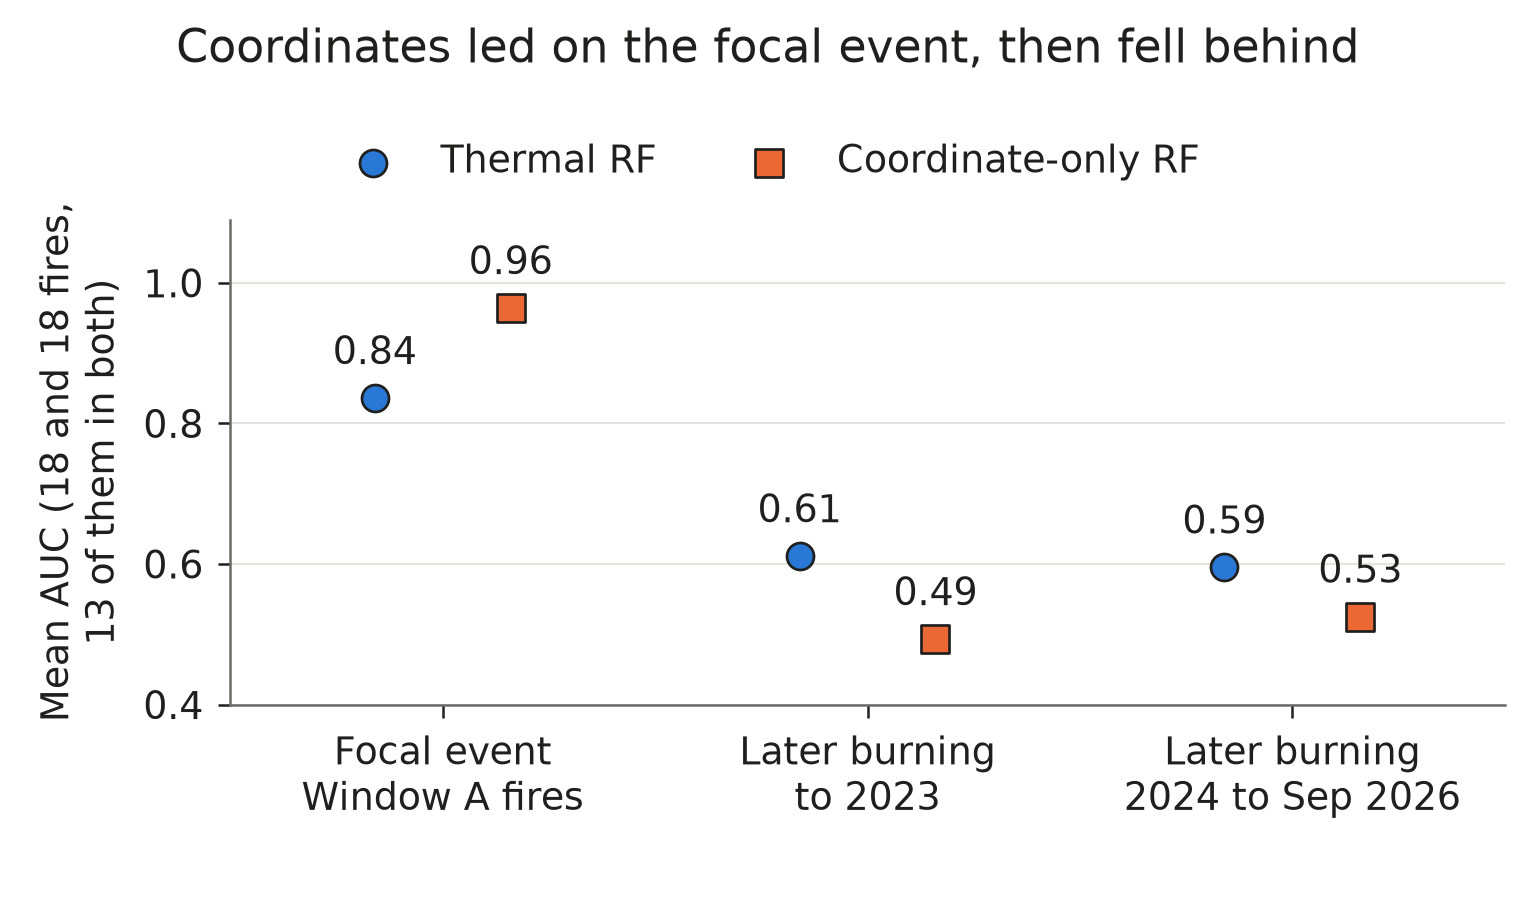
\includegraphics[width=\linewidth]{graphical_abstract.png}
\end{graphicalabstract}

\begin{highlights}
\item A coordinate-only forest beat a thermal forest on focal-fire AUC in \sAllCoordChose{} of \sAllN{} fires
\item Pooled AUC chose the coordinate-only forest in \sACrfChAuc{} of \sAElig{} fires with later burning
\item The choice cost \sACrfLossAuc{} AUC on burning to 2023 and \sBCrfLossAuc{} on burning in 2024-2026
\item The distance-calibrated AUC made the same choice in \sACrfChCauc{} of \sAElig{} fires
\item In simulations tuned to the real fires, all three measures chose near chance
\end{highlights}

\begin{keyword}
wildfire susceptibility \sep model selection \sep spatial cross-validation \sep temporal validation \sep random forest \sep MODIS burned area
\end{keyword}

\end{frontmatter}

\section{Introduction}
\label{sec:intro}

Maps of where wildfires are likely to burn are now mostly built with machine learning, trained on burned areas or ignitions mapped from satellites and judged by the area under the receiver operating characteristic curve (AUC) on held-out cells. A review of 298 machine-learning studies in wildfire science discussed the need for cross-validation suited to spatially autocorrelated data \citep{Jain2020}, and the best AUC reported in recent susceptibility studies is often above 0.9 \citep{Iban2022,Trucchia2023,Zerouali2026}. Blocking the cross-validation in space is the remedy recommended for such data \citep{Roberts2017}, and software for it is widely used \citep{Valavi2019}. Burned cells form contiguous patches, though, and a test block cut from the middle of one fire scar can still lie next to burned training cells. In species distribution modelling, \citet{Hijmans2012} showed that a predictor-free model scoring cells by their distance to training presences can match or beat environmental models. \citet{Bahn2007} found that spatial interpolation could outperform niche-based models, and \citet{Ploton2020} that a biomass model given only coordinates scored as well as one given environmental predictors under random validation. A high within-event AUC can therefore come from knowing where the scar is, with little help from the predictors.

A cross-validated AUC is rarely reported for its own sake. It is used to choose a model, a predictor set or a tuning, and the chosen model is then used to rank places where fire has not yet been seen. Whether that choice is the right one can only be checked against independent outcomes. In species distribution modelling, \citet{Baker2024} asked whether internal cross-validation picks the bias correction that does best on independent survey data, and \citet{Finn2024} compared the ranking of candidate models by internal AUC with their ranking on an independent field survey. \citet{Mila2024} used simulations with known prediction performance to test whether validation procedures rank random forests with and without spatial proxies correctly, and found that random cross-validation tended to favour the proxies in settings where they did not help. Hydrology has a similar line of work on whether calibration choices hold up on untouched periods \citep{Arsenault2018} and on the benchmarks a forecast has to beat \citep{Pappenberger2015}. In wildfire research, later burning has been used to evaluate maps. \citet{Trucchia2022} scored a summer susceptibility map of Italy against selected large fires of summer 2021, \citet{Moran2025} benchmarked annual burn probability maps against subsequent wildfires in California, and \citet{Preisler2008} compared fire probabilities with smoothed historic fire frequencies. \citet{PhelpsWoolford2021} set out how fire occurrence models should be evaluated and compared, and warned that an evaluation not matched to the operational use can select a model that is ineffective in that use. The studies we found do not report the loss incurred by choosing between two susceptibility models by their within-event cross-validated score, measured on the later burning that the models are meant to rank.

This paper measures that cost on 31 large Mediterranean fires mapped by MODIS. We fitted a random forest (RF) on thermal and environmental predictors (thermal RF) and a coordinate-only RF under 5~km block cross-validation. Three within-event measures chose between them, the pooled AUC, the calibrated AUC (cAUC) of \citet{Hijmans2012} and a distance-stratified version of it. We then scored both models on the burning that MODIS recorded in the same study rectangles after the focal fire. The first window runs to the end of 2023. The second, a replication with scores frozen before the labels were exported, runs from January 2024 to September 2026. Two hybrids that add coordinates or distance to training burns to the thermal RF test whether the result carries over to location features used in practice. A simulation in which the better model is known for each run tests how often each measure picks it. Section~\ref{sec:methods} describes the data, the models and the decision rules, Section~\ref{sec:results} the results, Section~\ref{sec:discussion} what they mean for model selection and Section~\ref{sec:conclusions} concludes.

\section{Data and methods}
\label{sec:methods}

The analysis needs fires with a burned label and predictors on a common grid, candidate models fitted under a fixed validation design, measures that choose between them on the focal fire and a later outcome against which the choice can be checked. Section~\ref{sec:fires} describes the fires and Section~\ref{sec:models} the candidate models. Section~\ref{sec:measures} defines the within-event measures, Section~\ref{sec:later} the later-burning labels and Section~\ref{sec:loss} the selection loss and the decision rules. Section~\ref{sec:sim} describes the simulation and Section~\ref{sec:order} the order in which the rules and the results were produced.

\subsection{Fires, cells and predictors}
\label{sec:fires}

The fires are five Mediterranean regions of an earlier study (Manavgat 2021, Bej\'is 2022, Mu\u{g}la 2021, North Evia 2021 and Montiferru 2021) and \vnAdded{} fires from 2017 to 2023 selected by rule from the MODIS MCD64A1 burned-area product \citep{MCD64A1,Giglio2018}. The rule took burned-area clusters of natural vegetation over the Mediterranean and kept those with a start between May and October, one dominant event and a rectangle of at most 1.1\textdegree{}. Clusters that overlapped one already chosen were dropped (\vselCandidates{} candidates, \vselPass{} after the filters, \vselKept{} kept, supplementary Section~S1). They are large single-event summer fires, and each study rectangle is drawn around one of them. For an added fire, a \vpredDays-day predictor window ends the day before the first burn date of the dominant event and a \vlabelDays-day label window starts on that day. The study rectangle is the extent of the labelled cells plus 0.15\textdegree{}. The five earlier regions keep the windows and rectangles of the earlier study. We call the fire whose burned area is the label the focal event.

All inputs were processed in Google Earth Engine \citep{Gorelick2017} by one open pipeline \citep{ThermalTwinRepo} and aggregated to cells of about 500~m. A cell is burned if MCD64A1 records a burn date inside the label window. The predictors are the Normalised Difference Vegetation Index (NDVI), elevation and slope from the Copernicus DEM \citep{CopernicusDEM}, land cover from the 2021 ESA WorldCover map \citep{Zanaga2022} and six thermal predictors from Landsat 8 \citep{LandsatC2L2} and MODIS MOD11A1 \citep{MOD11A1}. The thermal predictors are the land surface temperature (LST) of the predictor window, its anomaly against earlier years, a temperature-vegetation dryness index and its change, and a downscaled and a gap-filled LST. The population of each fire is the set of valid cells dominated by tree, shrub or grass cover in that map. For fires before 2021 the land cover postdates the predictor window, and for some it falls inside the later-burning window, so the analysis is retrospective and does not use only data available when a forecast would have been issued. The 31 fires hold between \vcellsMin{} and \vcellsMax{} such cells and \vburnedMin{} to \vburnedMax{} burned ones, and the burned share is \vprevMean\% on average (\vprevMin\% to \vprevMax\%). Supplementary Table~S1 lists the fires.

\subsection{Candidate models and validation}
\label{sec:models}

The model under evaluation is the thermal RF \citep{Breiman2001}, with 300 trees, a minimum leaf size of 3 and balanced class weights, trained on NDVI, elevation, slope, land cover and the six thermal predictors. Its main competitor is a coordinate-only RF with the same settings, whose two features are the coordinates of the cell centre in kilometres on the fire's grid. A $k$-nearest-neighbour classifier on the same coordinates ($k = 25$, distance-weighted, coordinate-only kNN) checks that the result is not specific to forests. Two hybrids represent location features that are used in practice. The first adds the two coordinates to the thermal RF. The second adds the distance to the nearest burned cell of the training folds, measured for training cells through an inner split by the same blocks so that the feature has the same geometry at training and at test time. A thermal RF without the six thermal predictors (baseline RF) is a secondary comparison.

Every model is fitted to each fire separately with five-fold cross-validation, stratified by label and grouped by blocks of 10 by 10 cells. A block is about 5~km north to south and somewhat less east to west, since cells are fixed in degrees. All models share the same folds and seed. The out-of-fold predictions of the five fold models are pooled into one score per cell. This is the map that a within-event evaluation scores, and it is also the map we score on later burning. It is not a single model trained on all cells of the fire.

\subsection{Within-event measures}
\label{sec:measures}

Three measures choose between two candidates on the focal event, each by the higher value. The pooled AUC is the ROC AUC of the pooled out-of-fold predictions. The cAUC follows \citet{Hijmans2012}. Inside each test fold, every burned cell with distance $d_p$ to the nearest burned training cell is paired with the unused unburned cell whose distance $d_n$ is most similar. The burned cells are taken in a seeded random order, and the pair is kept if $|d_n - d_p| \le 0.33 \max(d_p, 0.51\ \mathrm{km})$. The floor of 0.51~km, one cell, is our addition to the relative tolerance of \citet{Hijmans2012}. The kept pairs of all folds are pooled, and
\begin{equation}
\mathrm{cAUC} = \mathrm{AUC}_\mathrm{pairs} + 0.5 - \max(0.5, \mathrm{AUC}_\mathrm{null,pairs}),
\end{equation}
where the null model scores a cell by minus its distance to the nearest burned training cell. The null correction is the same for both candidates of a fire, so only the matching can make the cAUC choose differently from the pooled AUC. The stratified cAUC computes the AUC within strata of that distance, $[0, 0.51)$~km and then geometric strata whose bounds grow by a factor of 1.33. It averages the supported strata (at least 20 burned and 20 unburned test cells) with weights from the distance distribution of the burned test cells, renormalised over the supported strata. It is reported only if the supported strata cover at least 80\% of that distribution, and it is corrected by the null model in the same way as the cAUC. When a measure is not available for a fire or ties, no choice is recorded, and its loss is charged as if it had chosen the candidate that did worse on later burning.

The null model itself is not a candidate. Its AUC under the same folds shows how far closeness to burned training cells alone separates the classes in a given split, and we use it as a diagnostic of the split. When it is close to 1, the within-event test mostly asks whether a model can interpolate the scar.

\subsection{Later burning}
\label{sec:later}

Later burning is the burning that MCD64A1 version 6.1 recorded in the study rectangle after the focal label window. A cell is later-burned if at least half of its area has a burn date in the target window. Pixel-months without sufficient valid data (quality bit 1 clear, or no quality value) are counted, and cells in which more than 10\% of the pixel-months of the window lack valid data are left out of the population. The primary population is the model population of the fire minus the focal scar and minus these unmapped cells. Cells that burned before the target window stay in it. Window A runs from the end of the focal label window to 31 December 2023, so its length varies from fire to fire. Window B runs from 1 January 2024 to the last published month, September 2026. A fire is eligible in a window if it has at least 30 later-burned and 30 later-unburned cells in the primary population.

\subsection{Selection loss and decision rules}
\label{sec:loss}

For a fire and a pair of candidates, the loss of a measure is the AUC on later burning of the better candidate minus that of the candidate the measure chose. A measure that chooses the better model has no loss. Fires are weighted equally. Intervals come from a paired bootstrap over fires with 10,000 resamples and seed 42. Fires whose modelled cells have intersecting bounding boxes are resampled together as one cluster.

Two rules were fixed in advance. The first compares the pooled AUC with the cAUC through $D = L_\mathrm{pooled} - L_\mathrm{cAUC}$, the difference between their losses for the thermal and the coordinate-only RF. The cAUC is called better for this target if the lower end of the 95\% interval of the mean $D$ is above zero, and practically better if the mean $D$ is also at least 0.01 AUC. The two are called equivalent if the 90\% interval lies within $\pm 0.01$ AUC. The second calls a pair a transfer failure of within-event evaluation if the pooled AUC chooses the location-using candidate in at least 12 of 18 fires and the 95\% interval of the mean later-AUC difference (thermal RF minus candidate) is above zero. In window B the count threshold is $\lceil 12n/18 \rceil$ for $n$ fires, and every interval condition above zero is applied as a one-sided bootstrap $p < 0.025$. For each comparison these $p$ values are Holm-adjusted across the primary set and a secondary set, made of the eligible fires that were not eligible in window A. Equivalence keeps the unadjusted 90\% interval.

Sensitivities for the coordinate-only RF were set out with the first rule and are reported whatever they show. They are a two-year horizon, the full population with the focal scar included and equal weight per later fire event, where an event is an 8-connected component of later-burned cells grouped by an approximate year of first burning. They also include leaving out one event, one focal year or one fire at a time, and removing the largest later event of each fire. Leaving out one country was planned too, but countries were assigned to the 26 added fires only after the window-A results were known, and the $D$ of the distance hybrid was added at the same time. As a descriptive check we scored later burning by minus the distance to the focal scar, with an interval from 2,000 bootstrap resamples of fires. For three pairs of fires in which a later fire overlapped the rectangle of an earlier one, both RFs were trained on all cells of the earlier fire and scored on the later fire with its own predictors.

\subsection{Simulation}
\label{sec:sim}

Real later burning is a single realisation for each fire, so a simulation checks how often each measure picks the better model when the outcome can be generated anew. The landscapes are the population cells of the 31 fires with their real coordinates and predictors. A latent risk $\eta = aE + bS + \varepsilon$ has three parts. $E$ is an environmental index, the standardised mean of NDVI, minus elevation, slope and LST. $S$ is a Gaussian random field with exponential correlation of length $L$, and $\varepsilon$ is standard normal noise. The cells with the highest $\eta$ are burned, up to the real burned share of the fire. An environmental RF on the four signal predictors and two pure-noise predictors competes with a coordinate-only RF, both under the 5~km block design. The better model of a run is the one with the higher AUC on a second label of the same landscape, drawn once with the same $E$ and a new $S$ and $\varepsilon$. It stands for a later fire whose spatial footprint is not tied to the first one, and it is a realised ranking under this scenario, not an expected one.

The nominal design crosses $a \in \{0, 0.5, 1, 2\}$, $b \in \{0, 1, 2, 4\}$ and $L \in \{2, 10\}$~km, with \sSimTenDraws{} draws per fire and setting (\sSimTenAllRuns{} runs). It was repeated with one draw and 20~km blocks on the \sSimFortyFires{} fires large enough for them (\sSimFortyAllRuns{} runs). We report the runs with $b > 0$ (\sSimTenRuns{} and \sSimFortyRuns), since without a spatial field the two models have no spatial signal to differ on. A second design was tuned for each fire and each $a \in \{0.5, 1, 2\}$. Of 16 settings of $b \in \{2, 4, 8, 16\}$ and $L \in \{5, 10, 20, 40\}$~km, it kept the one whose null-model AUC and share of burned cells kept by matching came closest to fixed targets of 0.958 and 0.57 taken from the real fires, and then drew three new labels at that setting (\sSimCalRuns{} runs). For each measure we report its balanced accuracy against the truth and the mean AUC loss of its choice. Balanced accuracy is used because the environmental model is the truth in most nominal runs, so plain agreement would reward a measure that always picks it.

\subsection{Order of analysis}
\label{sec:order}

The analysis plan and its amendments are kept in the code repository (Section~\ref{sec:software}). An analysis register there records, for every reported result, when its rule was written relative to its own results and which time records are independent of the authors. The first rule of Section~\ref{sec:loss} was declared before any window-A score was compared with later burning, but after the within-event results and the simulations were known. The second rule was written after the window-A result for the coordinate-only RF was seen, so it is confirmatory only for the pairs whose results were still unseen (the hybrids and the coordinate-only kNN). For window B, the rules, the focal scores of all candidates and a SHA-256 manifest of those scores were pushed to the repository server on 15 November 2026, before the 2024 to 2026 labels were exported. The evaluation checked every score file against the manifest. Window B is therefore a frozen-score replication and not a blind test. The scores were frozen after the target period had passed, and per-fire counts of burned cells in those years had been read beforehand to set the eligibility rule. The pushes are recorded by the server, while the order of label export and evaluation between them rests on local file times and logs. The simulations and all other analyses are exploratory. Three analyses of the plan have no result. A forward selection that chooses between candidates by each site's own earlier fires had support at only two sites, and neither it nor its comparison with older fire labels produced a result file. Its sequence simulation was replaced by a later amendment before it ran. Supplementary Table~S4 lists every registered analysis with its status.

The labels of both windows were exported once more after all results were known. The first export excluded unmapped cells with bit 0 of the MCD64A1 quality layer, which is the land/water flag. An audit before submission found the error, and a plan amendment written before the new export replaced it with bit 1, the valid-data flag, leaving every other rule and the frozen scores unchanged. A check reproduced the original label of one fire exactly before the change. Over the 31 fires, the corrected mask removed \sQaCellsA{} cells (\sQaPctA\%) from the window-A populations, \sQaBurnedA{} of them later-burned, and \sQaCellsB{} (\sQaPctB\%) from window B, \sQaBurnedB{} of them later-burned. No fire changed eligibility. Refitting the location-using candidates in the rerun changed some AUC values in the eighth decimal place, which changed no reported value or choice. All results in the main text use the corrected labels, and supplementary Table~S3 sets them beside the original ones.

\section{Results}
\label{sec:results}

The results start with what the within-event test measures on these fires (Section~\ref{sec:res-diag}) and then follow the choice through the two windows of later burning (Sections~\ref{sec:res-a} and \ref{sec:res-b}). Section~\ref{sec:res-hybrid} reports the hybrids, Section~\ref{sec:res-sens} the sensitivities and Section~\ref{sec:res-sim} the simulation.

\subsection{What the within-event test rewards}
\label{sec:res-diag}

With 5~km blocks the null model reached a mean AUC of \vaucNullFive{} [\vaucNullFiveLo, \vaucNullFiveHi] against \vaucRfFive{} [\vaucRfFiveLo, \vaucRfFiveHi] for the thermal RF and scored higher in \vnullWinsFive{} fires. The coordinate-only RF reached a mean of \sAllFocCoord{} and scored higher than the thermal RF in \sAllCoordChose{} of \sAllN{} fires and higher than the null model in \sAllCoordBeatsNull{}. Distance matching kept \vpwdKeptFive\% of the burned cells on average, and on the kept pairs the null model still scored \vpwdNullFive{}. In these splits, closeness to burned training cells alone separated the classes better than the predictors did, and the coordinate-only RF learned the position of the scar from the coordinates.

\subsection{Selection and later burning to 2023}
\label{sec:res-a}

\sAElig{} fires had enough later burning in window A, and \sAExcl{} were left out, most of them fires of 2021 to 2023 with little time for later burning. In the eligible fires later burning came as a median of \sAEventsMed{} separate events (\sAEventsMin{} to \sAEventsMax), and the largest event held a median of \sALargestMed\% of the later-burned cells.

On the focal event the coordinate-only RF had a mean AUC of \sAFocCoord{} and the thermal RF \sAFocTherm{} in these fires, so the pooled AUC chose the coordinate-only RF in \sACrfChAuc{} of \sAElig{} fires (Table~\ref{tab:select}). The cAUC chose it in \sACrfChCauc{} and the stratified cAUC in \sACrfChSauc, the latter being unsupported in \sAUnsupSauc{} fires. On later burning the ranking reversed on average. The thermal RF had a mean AUC of \sALateTherm{} and the coordinate-only RF \sALateCoord, close to chance, and the thermal RF was better in \sACrfBetter{} fires, by \sACrfDiff{} [\sACrfDiffLo, \sACrfDiffHi] on average. The choice of the pooled AUC therefore lost \sACrfLossAuc{} AUC on average, which is \sACrfRel{} of the mean absolute difference between the two models on later burning. The baseline RF without thermal predictors reached a mean of \sABaseLate{} on the same later burning, so most of the gain over the coordinate-only RF comes from the environmental predictors as a whole. Scar exclusion does not explain the reversal either. With the focal scar kept in the population, the mean later AUC was \sAFullTherm{} for the thermal RF and \sAFullCoord{} for the coordinate-only RF. Fig.~\ref{fig:fires} shows the reversal fire by fire. The coordinate-only kNN gave the same picture, with a later-AUC difference of \sAKnnDiff{} [\sAKnnDiffLo, \sAKnnDiffHi]. Both pairs met the transfer-failure rule.

\begin{table}[t]
\centering
\caption{Choices on the focal event and their outcome on later burning, for the thermal RF against four location-using candidates. Chosen: number of fires in which the pooled AUC, the cAUC and the stratified cAUC chose the candidate. Better: fires in which the thermal RF had the higher AUC on later burning. Difference: mean AUC on later burning, thermal RF minus candidate, with 95\% bootstrap interval over fires. Loss: mean AUC loss of the pooled AUC's choice. Rule: transfer-failure rule of Section~\ref{sec:loss}. Window A has \sAElig{} fires and window B \sBElig, \sBOverlap{} of them in both.}
\label{tab:select}
\footnotesize
\setlength{\tabcolsep}{3pt}
\begin{tabular}{L{3.0cm}cccL{3.1cm}cc}
\toprule
Candidate & Chosen & Better & & Difference & Loss & Rule \\
\midrule
\multicolumn{7}{l}{\emph{Window A, later burning to 2023}} \\
Coordinate-only RF & \sACrfChAuc{} / \sACrfChCauc{} / \sACrfChSauc & \sACrfBetter & & \sACrfDiff{} [\sACrfDiffLo, \sACrfDiffHi] & \sACrfLossAuc & \sACrfRule \\
Coordinate-only kNN & \sAKnnChAuc{} / \sAKnnChCauc{} / \sAKnnChSauc & \sAKnnBetter & & \sAKnnDiff{} [\sAKnnDiffLo, \sAKnnDiffHi] & \sAKnnLossAuc & \sAKnnRule \\
Thermal RF + coordinates & \sATcChAuc{} / \sATcChCauc{} / \sATcChSauc & \sATcBetter & & \sATcDiff{} [\sATcDiffLo, \sATcDiffHi] & \sATcLossAuc & \sATcRule \\
Thermal RF + distance & \sATdChAuc{} / \sATdChCauc{} / \sATdChSauc & \sATdBetter & & \sATdDiff{} [\sATdDiffLo, \sATdDiffHi] & \sATdLossAuc & \sATdRule \\
\midrule
\multicolumn{7}{l}{\emph{Window B, later burning January 2024 to September 2026, frozen scores}} \\
Coordinate-only RF & \sBCrfChAuc{} / \sBCrfChCauc{} / \sBCrfChSauc & \sBCrfBetter & & \sBCrfDiff{} [\sBCrfDiffLo, \sBCrfDiffHi] & \sBCrfLossAuc & \sBCrfRule \\
Coordinate-only kNN & \sBKnnChAuc{} / \sBKnnChCauc{} / \sBKnnChSauc & \sBKnnBetter & & \sBKnnDiff{} [\sBKnnDiffLo, \sBKnnDiffHi] & \sBKnnLossAuc & \sBKnnRule \\
Thermal RF + coordinates & \sBTcChAuc{} / \sBTcChCauc{} / \sBTcChSauc & \sBTcBetter & & \sBTcDiff{} [\sBTcDiffLo, \sBTcDiffHi] & \sBTcLossAuc & \sBTcRule \\
Thermal RF + distance & \sBTdChAuc{} / \sBTdChCauc{} / \sBTdChSauc & \sBTdBetter & & \sBTdDiff{} [\sBTdDiffLo, \sBTdDiffHi] & \sBTdLossAuc & \sBTdRule \\
\bottomrule
\end{tabular}
\end{table}

\begin{figure}[t]
\centering
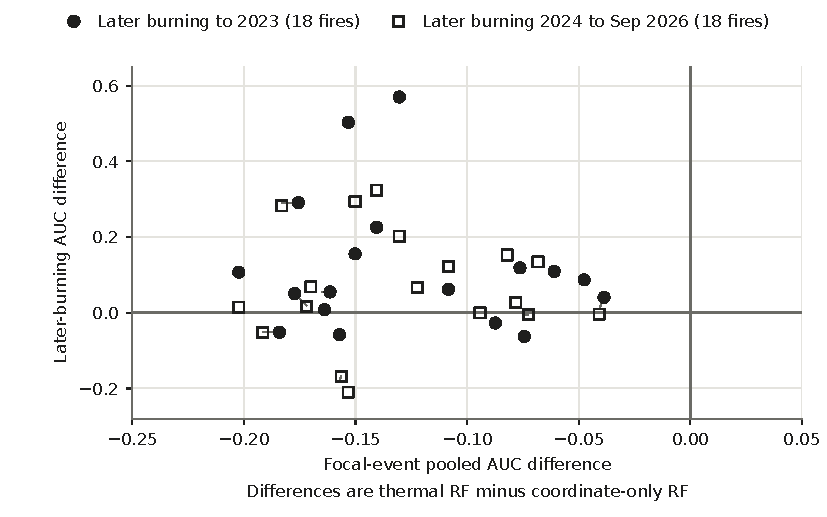
\includegraphics[width=0.85\linewidth]{figures/Figure_1.pdf}
\caption{Focal-event choice against outcome on later burning, one marker per fire and window. The horizontal axis is the pooled AUC of the thermal RF minus that of the coordinate-only RF under 5~km block cross-validation on the focal fire, so every marker left of the vertical line is a fire in which the pooled AUC chose the coordinate-only RF. The vertical axis is the same difference in AUC on later burning in the same study rectangle, so markers above the horizontal line are fires in which that choice was the worse one. Filled circles: later burning to the end of 2023. Hollow squares: later burning from January 2024 to September 2026, scored with frozen focal predictions. Where two markers would overlap, one is shifted slightly and joined to its true position by a short line.}
\label{fig:fires}
\end{figure}

The two calibrated measures did not change the outcome. The mean of $D$, the loss of the pooled AUC minus that of the cAUC, was \sADMean{} with a 90\% interval of [\sADLo, \sADHi]. This lies inside the margin of $\pm 0.01$, so the first rule called the two measures equivalent. They made the same choice in nearly every fire, and the mean cAUC of the coordinate-only RF (\sAFocCoordC) stayed above that of the thermal RF (\sAFocThermC). Between the thermal and the baseline RF the pooled AUC chose the thermal RF in \sABaseChoseTherm{} fires, and the baseline RF did better on later burning in \sABaseBetter{} of them, for a loss of \sABaseLossAuc. Between two models with the same kind of predictors the within-event choice was mostly right, and it went wrong when one candidate could learn the location of the scar.

\subsection{Replication on burning from 2024 to September 2026}
\label{sec:res-b}

\sBElig{} fires had enough later burning in window B, \sBOverlap{} of them also eligible in window A and \sBSec{} new (Table~\ref{tab:select}). The pooled AUC chose the coordinate-only RF in all \sBCrfChAuc, and on burning from 2024 the thermal RF was better in \sBCrfBetter{} fires, by \sBCrfDiff{} [\sBCrfDiffLo, \sBCrfDiffHi] on average (Holm-adjusted $p = \sBCrfP$). The mean AUC on later burning was \sBLateTherm{} for the thermal RF and \sBLateCoord{} for the coordinate-only RF, and the loss of the pooled AUC's choice \sBCrfLossAuc. The coordinate-only kNN gave a difference of \sBKnnDiff{} [\sBKnnDiffLo, \sBKnnDiffHi]. Both pairs met the transfer-failure rule again. In the \sBSec{} fires that had not been eligible in window A, whose later-burning scores had never been seen, the difference for the coordinate-only RF was \sBSCrfDiff{} [\sBSCrfDiffLo, \sBSCrfDiffHi], with the thermal RF better in \sBSCrfBetter. The pooled AUC and the cAUC were again equivalent (mean $D$ \sBDMean, 90\% interval [\sBDLo, \sBDHi]) and made the same choice in \sBDSame{} of \sBElig{} fires. The effect was smaller than in window A, and its interval came close to zero.

\subsection{Hybrid models}
\label{sec:res-hybrid}

Adding coordinates or the distance to training burns to the thermal RF also raised its within-event AUC, and the pooled AUC chose each hybrid over the plain thermal RF in all fires of both windows. On later burning the plain thermal RF was ahead on average, but by less (Table~\ref{tab:select}, Fig.~\ref{fig:pairs}). The hybrid with coordinates did not meet the transfer-failure rule in either window. The hybrid with distance did not meet it in window A and met it in window B with a Holm-adjusted $p$ of \sBTdPfour, just below the threshold of 0.025. With the original labels (Section~\ref{sec:order}) the same $p$ was \sOBTdP{} and the rule was not met, so this result sits on the threshold. For the thermal RF with coordinates the later-AUC difference was \sATcDiff{} [\sATcDiffLo, \sATcDiffHi] in window A and \sBTcDiff{} [\sBTcDiffLo, \sBTcDiffHi] in window B. For the thermal RF with distance it was \sATdDiff{} [\sATdDiffLo, \sATdDiffHi] and \sBTdDiff{} [\sBTdDiffLo, \sBTdDiffHi]. The cAUC behaved differently for this second hybrid. It chose the hybrid in only \sATdChCauc{} fires in window A and \sBTdChCauc{} in window B. Its loss was lower than that of the pooled AUC (\sATdLossCauc{} against \sATdLossAuc{} in window A), although the interval of the difference included zero (\sATdD{} [\sATdDLo, \sATdDHi]). In the \sBSec{} secondary fires of window B the distance hybrid met the rule with both label versions, with a difference of \sBSTdDiff{} [\sBSTdDiffLo, \sBSTdDiffHi], but five fires carry little weight. The selection result of this paper is clear for coordinate-only learners. For the distance hybrid it holds in one window and at the threshold, and for the coordinate hybrid it was not shown, so it does not extend to location features in general.

\begin{figure}[t]
\centering
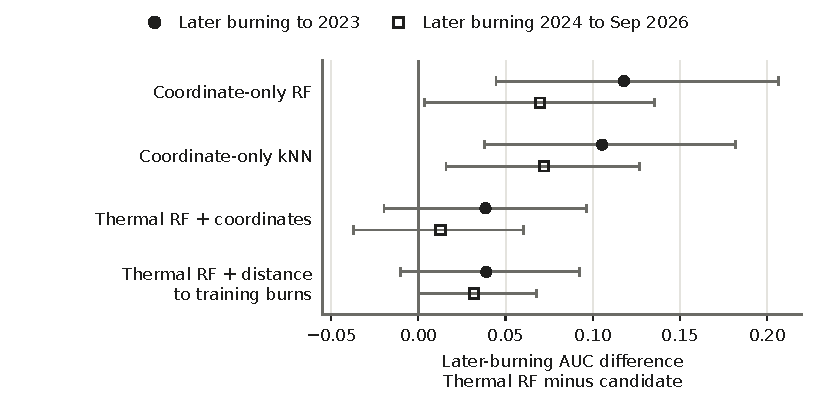
\includegraphics[width=0.85\linewidth]{figures/Figure_2.pdf}
\caption{Mean AUC on later burning of the thermal RF minus that of each location-using candidate, with 95\% bootstrap intervals over fires. Filled circles: later burning to the end of 2023 (\sAElig{} fires). Hollow squares: later burning from January 2024 to September 2026 (\sBElig{} fires). Values above zero mean that the thermal RF ranked later burning better. In both windows the pooled AUC chose the candidate in every fire.}
\label{fig:pairs}
\end{figure}

\subsection{Sensitivity}
\label{sec:res-sens}

For the coordinate-only RF in window A, $D$ stayed within the equivalence margin with the full population including the focal scar (\sADFull, 90\% interval [\sADFullLo, \sADFullHi]), with a two-year horizon (\sADTwoYear, \sATwoYearFires{} fires) and with equal weight per later event (\sADEvent). Leaving out one later event at a time moved the per-fire $D$ between \sALoeoMin{} and \sALoeoMax. The later-AUC difference stayed positive when one focal year was left out (\sALoyoMin{} to \sALoyoMax), one fire (\sALofoMin{} to \sALofoMax) or, in the check added later, one country (\sALocoMin{} to \sALocoMax{} over \sACountries{} countries). Removing the largest later event of each fire left \sANoLargestFires{} fires with enough burning, and the thermal RF was still better in \sANoLargestBetter{} of them, by \sANoLargest{} on average. Closeness to the focal scar ranked later burning weakly on average, with a mean AUC of \sAScar{} [\sAScarLo, \sAScarHi] for minus the distance to the scar and single fires from \sAScarMin{} to \sAScarMax. In the \sRpN{} pairs of overlapping fires, the pooled AUC on the earlier fire chose the coordinate-only RF in all \sRpCoordChosen, and the thermal RF trained on the earlier fire scored the later one better in \sRpThermBetter. The pairs overlap to very different degrees, and in one of them the two fires share almost no cells, so they are only illustrations (supplementary Table~S5). Supplementary Table~S2 gives the per-fire values of the two windows, and Table~S4 lists every analysis of the plan with its status and result.

\subsection{Simulation}
\label{sec:res-sim}

In the nominal design the cAUC picked the better model more often than the pooled AUC (Fig.~\ref{fig:sim}). Its balanced accuracy was \sSimTenBalCauc{} against \sSimTenBalAuc{} with 5~km blocks and \sSimFortyBalCauc{} against \sSimFortyBalAuc{} with 20~km blocks, and the stratified cAUC lay between them. Its mean AUC loss was \sSimTenLossCauc{} against \sSimTenLossAuc{} for the pooled AUC with 5~km blocks. In the design tuned to the real fires the advantage disappeared. The environmental model was the better one in \sCalEnvWon{} of \sSimCalRuns{} runs, yet the pooled AUC never chose it and the cAUC chose it \sCalCaucEnv{} time. In that run the coordinate model was in fact the better one. The stratified cAUC never chose it, with unsupported runs counted as failures. All three measures thus chose at about chance level (balanced accuracy \sSimCalBalAuc, \sSimCalBalCauc{} and \sSimCalBalSauc), with a mean loss of about \sSimCalLossAuc. A fixed rule that always picks the environmental model, which only a simulation can know to be the safer default, lost less than any measure (\sSimTenLossEnv{} and \sSimFortyLossEnv{} in the nominal designs, \sSimCalLossEnv{} in the tuned one). On average the tuned scenarios still fell short of the real fires. Their mean null-model AUC was \sCalNullSim{} against \sCalNullReal, matching kept \sCalKeptSim\% of the burned cells against \sCalKeptReal\%, and the stratified cAUC was supported in \sCalSupSim\% of runs against \sCalSupReal\% of the real fires. The real fires are thus on average a more extreme case than the tuned scenarios.

\begin{figure}[t]
\centering
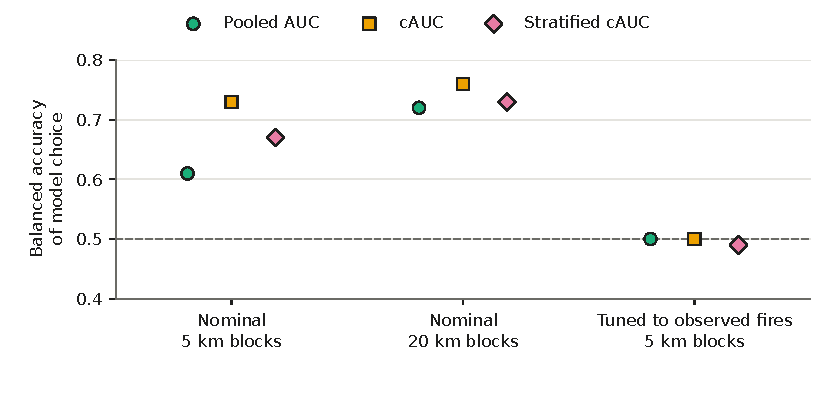
\includegraphics[width=0.85\linewidth]{figures/Figure_3.pdf}
\caption{Balanced accuracy with which three within-event measures chose the model that was better on an independent second label, in three simulation settings. Nominal: latent risk with a fixed grid of environmental and spatial weights, runs with a spatial weight $b > 0$ only (\sSimTenRuns{} runs with 5~km blocks, \sSimFortyRuns{} with 20~km blocks). Tuned: spatial weight and range set per fire and environmental weight so that the null-model AUC and the matched share came close to targets taken from the real fires (\sSimCalRuns{} runs). The dashed line marks a choice no better than chance.}
\label{fig:sim}
\end{figure}

\section{Discussion}
\label{sec:discussion}

On these fires, the within-event test rewarded the model that knew where the scar was, and that model ranked later burning worse in both windows. Section~\ref{sec:disc-why} discusses why, Section~\ref{sec:disc-lit} relates the result to earlier work, Section~\ref{sec:disc-rec} turns it into recommendations and Section~\ref{sec:disc-limits} gives the limits of the study.

\subsection{Why the within-event score points the wrong way}
\label{sec:disc-why}

With 5~km blocks inside one fire, closeness to burned training cells separated the classes with a mean AUC of \vaucNullFive, so a learner that can interpolate the scar scores high. The null model did so with no predictor, and the coordinate-only RF did slightly better in most fires, which fits its ability to learn the shape of the scar as well as its position. Later burning was scored outside the focal scar, and closeness to the scar ranked it with a mean AUC of only \sAScar. The coordinate-only RF carried the scar's geometry into a period in which that geometry mattered little, and its mean AUC on later burning was close to chance. The thermal RF ranked later burning better than the coordinate-only RF, but only slightly better than the baseline RF without thermal predictors in window A (\sALateTherm{} against \sABaseLate) and about equally in window B (\sBLateTherm{} against \sBBaseLate). What carried over to later fires is thus a weak environmental signal, and these data do not single out the thermal predictors. The cAUC and its stratified version did not repair the choice. Their null correction shifts both candidates equally, so only the matching or the strata could change the order, and on these splits the coordinate-only RF kept the higher cAUC in \sACrfChCauc{} of \sAElig{} fires.

The simulation agrees with this reading without proving it. In the nominal scenarios the cAUC chose better than the pooled AUC, as \citet{Hijmans2012} intended. In the scenarios tuned towards the spatial separation of the real fires, the measures almost never chose the environmental model and their choices were at about chance level. The averages do not locate a threshold at which the cAUC stops helping, but they show that its benefit seen in the nominal settings did not carry over to settings resembling these fires.

\subsection{Relation to earlier work}
\label{sec:disc-lit}

The selection question is not new. \citet{Baker2024}, \citet{Finn2024} and \citet{Mila2024} checked choices made by internal validation against independent data or simulated truth, and \citet{Mila2024} found that random cross-validation favours spatial proxies in settings where they do not help. Our fires add three things to that picture. The outcome is real later burning in the same areas, in two windows, the second one scored with frozen predictions. The within-event split is spatial block cross-validation, the remedy recommended for spatial dependence \citep{Roberts2017}, and the calibrated AUC of \citet{Hijmans2012} is included as a selector. The simulations show that the advantage of the calibrated measure in nominal settings did not hold in settings tuned towards the real fires. The coordinate-only learner is close to the interpolators that \citet{Bahn2007} and \citet{Ploton2020} used as references, and our results agree with theirs that such learners can match or beat environmental models within the sampled area.

For wildfire, evaluation against later burning is established \citep{Verde2010,Trucchia2022,Moran2025}, and \citet{PhelpsWoolford2021} recommended evaluation designs matched to the intended use of a model, warning that a mismatched evaluation can select an operationally ineffective one. Our results put a size on that warning for one common design, since the within-event score and the score on later burning pointed to different models.

\subsection{Recommendations}
\label{sec:disc-rec}

Three practices follow from the results. First, when a susceptibility map is meant to rank where future fires will burn, candidate models should be chosen on later burning. This needs a temporal hold-out in which the training data end before the target period starts. Within-event cross-validation can still serve to check a model, but on our evidence its AUC should not decide between an environmental model and one that can learn location from coordinates alone. For hybrids the evidence is weaker, and a temporal hold-out is the safer basis for that choice too. Second, studies should report the AUC of the predictor-free null model under their own split. It costs one nearest-neighbour query per fold, and a value close to 1 shows that the within-event test mostly rewards interpolation of the scar. Third, the cAUC should not be relied on to correct the choice in such splits. In our fires it made the same choice as the pooled AUC in nearly every case, while in simulations with weaker spatial separation it helped. A selection made on later burning needs no correction of this kind. The analysis code computes all three within-event measures and the later-burning loss for any set of fires with burned-area labels (Section~\ref{sec:software}).

\subsection{Limitations}
\label{sec:disc-limits}

Window A has \sAElig{} eligible fires and window B \sBElig, of which \sBOverlap{} are shared, so the two windows are not independent replications, and window B is a frozen-score replication run after its target period had passed. The direction held on average, but in single fires the coordinate-only RF did better on later burning in \sACrfCoordBetter{} of \sAElig{} fires in window A. Eligibility required at least 30 later-burned and 30 later-unburned cells, which an operational user cannot know in advance, so the results are conditional on later burning having occurred. Window A leans on fires of 2017 to 2021, because more recent fires had little time to reburn nearby. Later burning came in few events per fire and is a single realisation of weather and ignitions, not the underlying susceptibility. The results held when the largest event was removed, but a few events still weigh heavily in each fire, and the year used to group later burning into events is approximate. The scored map is assembled from five fold models and is not an operational model trained on all cells. The land cover predictor and population mask come from a 2021 map, so the analysis is retrospective. The validation of the previous MCD64A1 collection showed that a 500~m product misses small fires and partly burned cells \citep{Boschetti2019}. The fires are large single-event summer fires with rectangles drawn around them, and the results may not hold for regional inventories of many small fires.

The comparison is limited to AUC on later burning. We did not score calibrated probabilities with proper scoring rules, and we did not compare the candidates with a reference built only from the fire history of each landscape. Both are needed before the thermal RF can be called useful for forecasting, since a better rank than the coordinate-only RF does not show skill against simpler references. The selection rule of the first window was written after the within-event results were known, the transfer-failure rule after the coordinate-only result of that window, and the simulations are exploratory. The tuned simulation did not reach the spatial separation of the real fires.

\section{Conclusions}
\label{sec:conclusions}

Within-event spatial block cross-validation on 31 Mediterranean fires preferred a coordinate-only random forest to a forest on thermal and environmental predictors in every fire. On the burning that followed in the same areas, in two sets of \sAElig{} and \sBElig{} eligible fires, the choice cost a mean of \sACrfLossAuc{} AUC to the end of 2023 and \sBCrfLossAuc{} from 2024 to September 2026. The calibrated AUC of \citet{Hijmans2012} made the same choice in \sACrfChCauc{} of \sAElig{} fires in window A and \sBCrfChCauc{} of \sBElig{} in window B. For hybrids that add location to the thermal predictors the evidence was weaker. Only the distance hybrid met the declared rule, in window B and at the threshold. Model selection for susceptibility maps that will rank future burning should therefore use later burning, and the null-model AUC of the split should be reported to show how much a within-event score rewards interpolation. The next steps are a comparison with fire-history references under proper scores and a selection test in landscapes and seasons whose outcomes are unknown when the choice is fixed.

\section*{Software and data availability}
\label{sec:software}

Software name: thermal-twin analysis code (branch scaleup-31fires). Developers: Y.E. Cogurcu and E. Metin, ycogurcu@cu.edu.tr. First available: 2026. Hardware: a desktop computer with 32 threads. Software required: Python 3.12 with NumPy, pandas, SciPy, scikit-learn, rasterio and the Earth Engine Python API. Programming language: Python. Availability and cost: free, MIT licence, at \url{https://github.com/dryuemco/thermal-twin}. The analysis plan, its amendments and the analysis register are in the same repository. The upstream processing pipeline is at \url{https://github.com/emrehann17/satellite-thermal-digital-twin}. All satellite inputs are public and were accessed through Google Earth Engine. The modelling tables of the 31 fires, the later-burning labels, the frozen focal scores with their SHA-256 manifest and the outputs behind every figure and table will be archived with the code in a versioned Zenodo release before publication.

\section*{CRediT authorship contribution statement}

Emrehan Metin: Software, Data curation, Investigation, Validation, Writing -- review and editing. Yunus Emre Cogurcu: Conceptualization, Methodology, Formal analysis, Investigation, Visualization, Writing -- original draft, Writing -- review and editing, Supervision, Project administration, Funding acquisition.

\section*{Declaration of competing interest}

The authors declare that they have no known competing financial interests or personal relationships that could have appeared to influence the work reported in this paper.

\section*{Funding}

This work was supported by the \c{C}ukurova University Scientific Research Projects Coordination Unit under project FKB-2025-17608. The funder had no role in the study design, the analysis, the writing or the decision to submit.

\section*{Acknowledgements}

The authors thank the Department of Computer Engineering at \c{C}ukurova University for the laboratory environment in which this work was carried out.

\section*{Declaration of generative AI and AI-assisted technologies in the manuscript preparation process}

During the preparation of this work the authors used Claude (Anthropic) and Codex (OpenAI) to write analysis and figure code, to run analysis scripts, to check reported numbers against the result files, to review the design and to draft and edit the text. After using these tools, the authors reviewed and edited the content as needed and take full responsibility for the content of the published article.

\bibliographystyle{elsarticle-harv}
\bibliography{references}

\end{document}
